\documentclass[12pt,a4paper]{article}

\usepackage[utf8]{inputenc}
\usepackage[spanish,english]{babel}
\usepackage[T1]{fontenc}
\usepackage{amsmath, amssymb, amsfonts}
\usepackage{amsthm}
\usepackage{geometry}
\usepackage{graphicx}
\usepackage{booktabs}
\usepackage{caption}
\usepackage{enumitem}
\usepackage{float}
\usepackage{tikz}
\usepackage{pgfplots}
\usepackage[authoryear]{natbib}
\usepackage{hyperref}
\usepackage{threeparttable}
\usepackage[english]{cleveref}
\pgfplotsset{compat=1.17}

\geometry{margin=1in}

% Theorem Definitions
\newtheorem{proposition}{Proposition}
\newtheorem{corollary}{Corollary}
\newtheorem{definition}{Definition}
\newtheorem{lemma}{Lemma}
\theoremstyle{remark}
\newtheorem{remark}{Remark}
\newtheorem{condition}{Condition}

% Fix Unicode characters
\DeclareUnicodeCharacter{2264}{\ensuremath{\leq}}

% Define argmax command
\DeclareMathOperator*{\argmax}{arg\,max}

\begin{document}

\title{A Real-Time Forecasting-Ensemble Index of Economic Uncertainty and the Volatility of GDP Revisions}
\author{Manuel Hidalgo-Pérez\thanks{Universidad Pablo de Olavide. Email: mhidper@upo.es} \and Leandro Navarro Pablo\thanks{Autoridad Independiente de Responsabilidad Fiscal (AIReF). Email: leandro.navarro@airef.es}}
\date{}

\maketitle

\begin{abstract}
Statistical agencies face a fundamental trade-off between timeliness and accuracy, particularly during economic crises when real-time data becomes structurally disordered. We ask whether the dispersion and instability of a real-time forecasting ensemble anticipate the magnitude of subsequent revisions in official GDP figures, and whether this signal adds information beyond established uncertainty proxies. We construct a Composite Economic Uncertainty Index (CEUI) from three real-time dimensions of a five-model ensemble (VAR, Random Forest, ARIMA, LSTM, and Dynamic Factor Models)---within-model variability, between-model dispersion, and temporal instability---applied to Spanish GDP growth over 2015Q4--2024Q4. The index, computed under an expanding-window protocol that uses only data dated up to each quarter (a quasi-real-time design), is strongly associated with the magnitude of subsequent revisions $(\rho = 0.727, p < 0.001)$. In a horse-race against the VIX and the Economic Policy Uncertainty (EPU) index for Spain, the CEUI carries predictive information about data quality that the external proxies do not: it remains significant at the 1\% level while the VIX and EPU become insignificant once it is included. The results suggest that the internal disorder of a forecasting system is a useful real-time leading indicator of the reliability of official statistics.

\vspace{0.5cm}
\noindent\textit{JEL codes:} C53, C82, E01, E32.\\
\textbf{Keywords:} Economic Uncertainty, Forecast Combinations, Informational Entropy, GDP Revisions, Real-time Data.
\end{abstract}


\section{Introduction}

Modern macroeconomics and policy design rely heavily on the prompt availability of National Accounts. However, statistical agencies such as Spain's INE (\textit{Instituto Nacional de Estadística}) face an inherent trade-off between timeliness and precision \citep{mankiw1986}. The production of ``flash'' GDP estimates requires statistical triangulation under conditions of incomplete information, leading to substantial ex-post revisions as newer and more comprehensive data becomes available. While revisions are a natural part of the statistical production cycle, their magnitude and direction are not uniform over time. As \citet{orphanides2001} noted, utilizing real-time data that is prone to large subsequent revisions can lead to significant policy missteps, particularly in real-time macroeconomic calibration and monitoring.

Recently, global disruptions---the 2008 financial crisis, the European sovereign debt crisis, and the COVID-19 pandemic---have highlighted that this timeliness-accuracy trade-off is drastically amplified during periods of economic stress. In stable regimes, revisions to Spanish GDP growth are relatively small. However, the magnitude of these corrections (Mean Absolute Error, MAE) spikes by amplification factors of 1.5x during the Global Financial Crisis, 1.7x during the Sovereign Debt Crisis, and 2.8x during the COVID-19 pandemic compared to normal periods. 

To systematically track this instability, we measure revision volatility ($\sigma^{rev}_t$) as the standard deviation of the successive updates made to the initial ``flash'' GDP estimate of quarter $t$ over the subsequent two years. \Cref{fig:volatility_ts} illustrates the temporal evolution of this metric in Spain, confirming that during major crises, statistical agencies are not merely dealing with missing data, but with a structural breakdown of the informational environment.

\begin{figure}[ht]
    \centering
    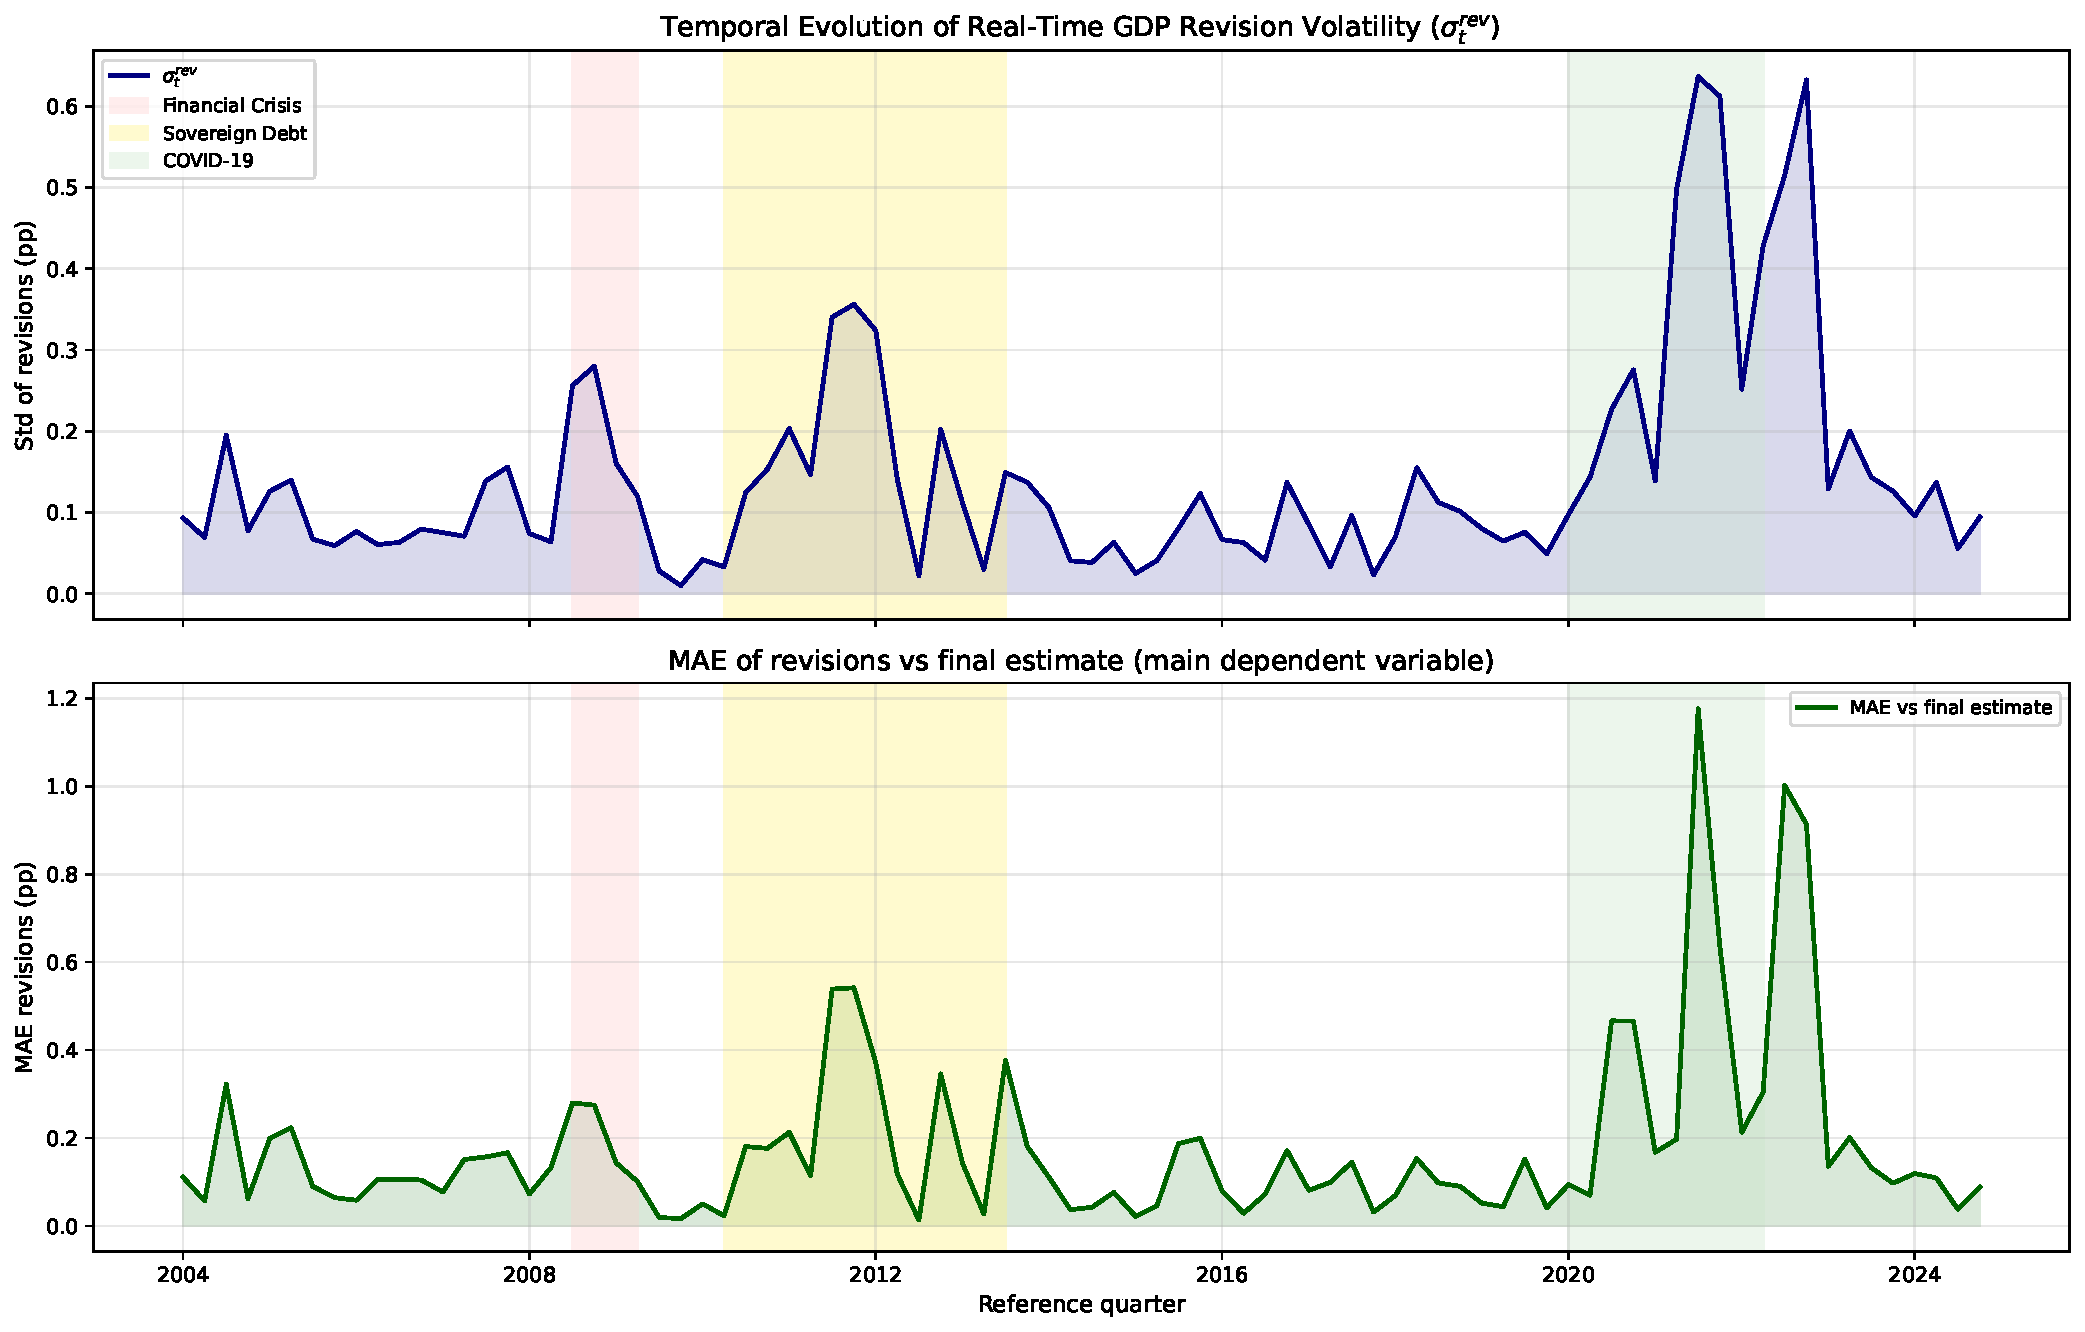
\includegraphics[width=0.85\textwidth]{figures/fig1_revision_volatility.pdf}
    \caption{Temporal Evolution of Real-Time GDP Revision Volatility ($\sigma^{rev}_t$) in Spain (2005--2024). The shaded areas represent major crisis episodes: the Global Financial Crisis (2008--2009), the European Sovereign Debt Crisis (2010--2012), and the COVID-19 pandemic (2020--2022).}
    \label{fig:volatility_ts}
\end{figure}

Despite the well-documented existence of these revision spikes \citep{pavia2018, croushore2011}, the precise mechanism through which economic uncertainty translates into statistical error remains largely unmeasured. The revision literature and the uncertainty measurement literature have advanced in parallel but without a formal bridge connecting them. This paper provides that bridge by formalizing the link between the internal disorder of a forecasting system and the quality of official statistics.

We hypothesize that the magnitude of revision errors reflects the informational disorder prevalent at the time of the initial estimate. Rather than pursuing a formal information-theoretic proof, our approach is strictly operational. We measure this disorder by aggregating three observable dimensions of predictive ambiguity within a forecasting ensemble, capturing average internal model dispersion, disagreement among competing modelling paradigms, and the instability of forecasts between consecutive periods. The theoretical motivation for this decomposition is outlined in Appendix~A.

Our contribution is primarily empirical. First, we provide a framework that maps the internal statistics of a forecasting ensemble to observable, real-time measures of predictive ambiguity, functioning entirely without look-ahead bias. Second, we extend the analysis of National Accounts quality in Spain \citep{pavia2018}, documenting the evolution of revision patterns through recent crisis episodes. Third, we establish the CEUI as a leading indicator of data-quality variation that improves on standard macroeconomic uncertainty proxies. Over the 2015Q4--2024Q4 evaluation window ($N = 37$ quarters), the Spearman rank correlation between the index and revision volatility is $\rho = 0.727$ ($p < 0.001$). Estimating our baseline specification yields a positive slope, $\hat{\beta} = 0.0198$, significant at the 1\% level, with $R^2 = 0.413$. In a horse-race against the VIX and the Economic Policy Uncertainty (EPU) index for Spain, the CEUI carries predictive information about data quality that the external proxies do not, remaining significant at the 1\% level while the VIX and EPU become insignificant once it is included.

The results suggest that the dispersion across models and the instability of revisions observed in institutional forecasting are not merely noise but informative signals about the underlying reliability of real-time macroeconomic data. For producers and users of statistics, our index provides an ex-ante measure of the level of caution that should be applied to current estimates before committing to major economic decisions.

The remainder of the paper is structured as follows. \Cref{sec:lit_review} reviews the literature on data revisions and uncertainty measurement. \Cref{sec:data_revision} describes the real-time data vintages, the target variable, and the revision process. \Cref{sec:ceui_index} outlines the construction of the real-time uncertainty index. \Cref{sec:correlation_volatility} evaluates the empirical correlation of the CEUI with revision volatility, including a horse-race against external benchmarks. \Cref{sec:robustness} provides robustness checks, \Cref{sec:discussion} discusses the findings, and \Cref{sec:conclusion} concludes.

\section{Literature Review and Methodological Context}
\label{sec:lit_review}

Preliminary macroeconomic estimates are not random approximations to the truth. They are produced under institutional and informational constraints that introduce predictable, systematic patterns. The intuition that early data would simply be refined as more information arrives turns out to be empirically weak. Preliminary releases of GDP and monetary aggregates contain systematic departures from rationality, tending toward downward bias, excessive reliance on simple extrapolations of recent trends, and over-sensitivity to real-time seasonal adjustment procedures \citep{mankiw1986, mankiw1984, mork1987, kavajecz1995}. Revision errors, then, are not a minor calibration problem but a deeper structural friction between what agencies can measure promptly and what they eventually know to be true.

This friction was recognized early. \citet{howrey1978} showed formally that ignoring the distinction between preliminary and revised data when estimating econometric models leads to sub-optimal forecasts and unnecessarily large forecast errors. The finding that treating preliminary data as if it were final introduces a systematic handicap has since been confirmed across different national contexts. In a cross-country comparison of G-7 nations, \citet{faust2005} showed that subsequent GDP revisions can be predicted using variables that were already available at the time of the first release, implying that statistical agencies do not incorporate all existing information into their initial estimates and that these estimates are therefore systematically improvable. Similarly, \citet{fixler2002} documented persistent reliability challenges in US national accounts, especially around cyclical turning points, precisely the moments where policy relies most heavily on fresh data.

The production process itself is part of the explanation. Reconciling national accounts across different measurement approaches (income, expenditure and output) is a technically complex and lagged procedure. Achieving consistency between preliminary sectoral time series and benchmark revisions requires sophisticated statistical adjustments that mechanically generate corrections to earlier estimates \citep{chen2018}. A non-trivial share of GDP revisions is therefore not informational; it is a by-product of the accounting architecture of national statistics.

Revision errors do not behave uniformly over time. They are persistent and heteroscedastic, with a variance that fluctuates according to the macroeconomic regime. This is arguably the most policy-relevant finding in the revision literature, because the very moments when decision-makers most need reliable real-time data are precisely the moments when that data is least reliable.

\citet{aruoba2008} demonstrated this rigorously, showing that US data revisions violate the assumptions of standard state-space models and exhibit structural heteroscedasticity. For Spain, \citet{pavia2018} documented systematic seasonal patterns and clear regime dependence in the quality of GDP estimates. The trade-off between timeliness and accuracy worsens dramatically during episodes of economic stress. As \citet{asimakopoulos2023} have argued recently, the incentives facing statistical agencies create a structural bias toward publishing timely but less accurate estimates, and this bias becomes especially costly in crisis periods when the informational environment deteriorates most sharply.

This heteroscedasticity is not a statistical nuisance. It is the empirical motivation for our paper. If revision errors are systematically larger during periods of elevated uncertainty, there ought to be a real-time signal, computable ex ante, that tracks that variation. Finding and validating such a signal is the central contribution of this work.

Parallel to the revision literature, macroeconomics has invested heavily in building aggregate measures of uncertainty. The progression has been logical, moving from financial market proxies such as the VIX \citep{bloomuncer}, to macroeconomic indices that summarize the common unpredictable component across hundreds of series \citep{jurado2015}, and then to policy-based composite indices that combine newspaper coverage, tax code expiration dates and forecaster disagreement \citep{baker2016measuring}. For Spain, \citet{ghirelli2019} constructed a domestically calibrated version of the EPU index, showing that uncertainty measured this way correlates with investment slowdowns and GDP contractions.

These measures have proved valuable in macroeconomic research, but they share a common blind spot. They are designed to capture generalized economic risk, not the specific informational disorder that makes official statistics unreliable. The VIX signals market stress. The EPU captures policy ambiguity. Neither is designed to measure how much we should trust the most recent GDP flash estimate. \citet{berge2020} showed that real-time estimates of the output gap are subject to time-varying uncertainty that follows the business cycle, a finding closer to our concern, but even there the focus is on parameter uncertainty in a single model, not on the dispersion across a forecasting ensemble.

The most promising strand of uncertainty research, for our purposes, is the one focused on forecaster disagreement. The idea that the cross-sectional dispersion of professional forecasts contains information about aggregate uncertainty, beyond what a single model would indicate, has a long intellectual history \citep{mankiw2004}. The formal justification was provided by \citet{lahiri2010}, who showed, through a decomposition of forecast errors into common and idiosyncratic components, that total forecast uncertainty is exactly equal to inter-forecaster disagreement plus the variance of future aggregate shocks. Disagreement is therefore a theoretically grounded component of epistemic ambiguity, not an empirical curiosity. Nevertheless, disagreement-based measures rely on surveys (such as the Survey of Professional Forecasters or Consensus Economics), which are infrequent, subject to behavioral biases, and structurally limited to the set of forecasters who choose to participate \citep{clark2017, carriero2018}. An objective, model-based alternative is preferable for real-time monitoring purposes.

Taken together, the two strands reviewed above point to a gap that neither has filled. The revision literature documents \textit{that} official data degrades during crises. The uncertainty literature documents \textit{that} economic uncertainty rises during crises. But the formal, operational connection between the two, a real-time ex-ante index that predicts ex-post data quality, has not been established.

The conceptual roots of this gap run deep. \citet{knight1921} distinguished between risk, where the probability distribution of outcomes is known and can be priced, and genuine uncertainty, where the distribution itself is unknown. In stable periods, forecasting systems operate essentially in the risk domain, with models agreeing on the likely trajectory of the economy and revisions to preliminary estimates remaining modest. In episodes of acute macroeconomic stress, the environment shifts toward what \citet{ellsberg1961} called ambiguity, a state in which models diverge, agents cannot agree on the relevant probability model, and the informational basis of any estimate collapses. This transition is precisely what generates the revision spikes documented in \Cref{sec:data_revision}.

Formalized as an information-theoretic problem, the disorder of a forecasting system can be measured through entropy. Shannon entropy quantifies the spread of probability mass across possible outcomes, so that higher entropy corresponds to more disorder, less predictability, and, we argue, less trustworthy preliminary data. This approach has historical precursors in macroeconomics. \citet{patterson1991} applied informational entropy to characterize how uncertainty diminishes as national accounts are revised over successive vintages. More recently, \citet{shoja2017} showed that entropy-based measures are empirically superior to standard variance-based measures for capturing the meaningful disagreement among economic forecasters, since they are sensitive to the full shape of the distribution, not just its second moment. Methodologically, our construction of a composite entropy index from a multi-model ensemble relates to the frontier of forecast combination under uncertainty, where entropy has also proven to be an effective weighting criterion \citep{breto2019}.

Our framework operationalizes this intuition by constructing the CEUI, a composite real-time uncertainty index built from three dimensions of ensemble disorder (within-model variability, between-model dispersion, and temporal forecast instability). Unlike the unidimensional uncertainty proxies reviewed above, the CEUI is computable at the moment the flash estimate is published, is free of the full-sample normalisation bias common to composite indices, and is designed specifically to predict the subsequent magnitude of data revisions. The empirical validation of this link, and its superiority over the VIX and the EPU as predictors of Spanish GDP data quality, is the subject of \Cref{sec:correlation_volatility,sec:robustness}.


\section{Data and the Revision Process}
\label{sec:data_revision}

\subsection{CNTR Vintage Dataset}
Our primary dataset for the revision analysis is the real-time database of Spain's \textit{Contabilidad Nacional Trimestral} (CNTR), obtained from the INE. The dataset comprises a vintage triangle of quarterly observations, with publication vintages identified by their exact release timestamps. Each vintage corresponds to an official CNTR publication and contains the full historical GDP level series at that point in time.

The target variable is the year-on-year (YoY) GDP growth rate (seasonally adjusted), computed as the percentage change in the GDP level index relative to the same quarter of the preceding year. All revision metrics are computed on this growth rate series. We model the GDP growth rate on a YoY basis rather than a quarter-on-quarter (QoQ) basis. YoY growth is the preferred headline metric for Spanish macroeconomic monitoring, as it naturally filters out short-term quarterly noise and seasonal adjustments, making our linear estimations more stable and easier to interpret. However, since QoQ analysis is also of interest to capture high-frequency dynamics, we provide a complete set of results under a QoQ specification in Appendix~\ref{sec:appendix_qoq} as a robustness check. We show there that our qualitative findings and the predictive power of the CEUI are virtually unchanged.

We define two operationally precise concepts. The \textbf{flash estimate} ($y_{t,\text{flash}}$) is the first vintage published after the reference quarter $t$ has ended. The \textbf{final estimate} ($y_{t,\text{final}}$) is the most recent vintage available for each quarter. The \textbf{revision} for quarter $t$ is defined as $r_t = y_{t,\text{final}} - y_{t,\text{flash}}$. For the cross-sectional volatility analysis, we define the \textbf{revision standard deviation} $\sigma^{\text{rev}}_t$ as the standard deviation of all available vintage estimates for quarter $t$. This metric uses the full information content of the vintage triangle and is the key dependent variable in our regressions.

\subsection{Replication and Extension of Pav\'ia et al.\ (2018)}
\label{sec:pavia_results}

Table~\ref{tab:revision_errors} presents revision error statistics for the 2004--2024 period, computed over a two-year window from each quarter's first publication using the harmonised \texttt{cntr2} vintage triangle (base year 2015, 106 vintages). The seasonal pattern identified by \citet{pavia2018} is broadly confirmed, though Q3 now exhibits the highest MAE (0.266 pp), reflecting the concentration of large upward revisions during the COVID-19 recovery phase when the INE progressively incorporated new information about the rebound in activity.

\begin{table}[t]
\centering
\caption{Revision Error Statistics by Quarter (2004--2024)}
\label{tab:revision_errors}
\begin{tabular}{lccc}
\toprule
Quarter & Mean Error & MAE & Obs \\
\midrule
Q1 & -0.012 & 0.123 & 21 \\
Q2 & 0.005 & 0.111 & 21 \\
Q3 & 0.045 & 0.266 & 21 \\
Q4 & -0.007 & 0.226 & 21 \\
Average & 0.008 & 0.182 & 84 \\
\bottomrule
\end{tabular}
\end{table}


While the seasonal pattern is qualitatively similar to \citet{pavia2018} with respect to the high revision volatility in the third quarter (Q3), our findings differ in the fourth quarter (Q4). While \citet{pavia2018} reported a Q4 mean absolute revision error of virtually zero (0.00~pp), our calculations indicate a substantial MAE of 0.226~pp over the full sample, making Q4 the second most volatile quarter in terms of revisions. To understand this discrepancy, we perform a sub-sample analysis and examine the historical timeline of Spanish National Accounts. 

First, the inclusion of the COVID-19 pandemic (2020--2022) introduces massive volatility that distorts the full-sample averages; during this period, Q3 and Q4 MAEs reached 0.821~pp and 0.550~pp, respectively. However, even when restricting the analysis to the pre-COVID period (2004--2019), the MAE of Q4 remains high at 0.159~pp (compared to 0.174~pp in Q3, 0.116~pp in Q1, and 0.091~pp in Q2). 

Second, the Spanish statistical office (INE) implemented two major historical benchmark revisions (\textit{Cambios de Base}) after the publication of \citet{pavia2018}: Base 2015 (introduced in 2019) and Base 2021 (introduced in 2024). These benchmark revisions systematically updated the entire historical series, introducing retroactive corrections to Q4 levels that were absent in Pavía's original 1995--2016 sample. Recalculating the MAE over Pavía's exact reference period (1995--2016) using our current dataset reveals that Q4's retroactive MAE increases to 0.443~pp. 

Finally, a close inspection of Table~3 in \citet{pavia2018} suggests a mathematical anomaly: they report an interannual Q4 revision error of 0.00~pp for A0 (the initial flash or \textit{Avance} estimate) vs. DEF (the final definitive estimate), but simultaneously report Q4 errors of 0.18~pp for A1 (the first provisional revision) vs. DEF and 0.27~pp for A2 (the second provisional revision) vs. DEF. Given that the difference between A0 and A1 is only 0.01~pp, a zero revision for A0 vs. DEF is mathematically incompatible with a large revision for A1 vs. DEF under the triangle inequality. Moreover, their interquarterly Q4 revision error was reported as 0.33~pp. Taken together, these points clarify that Q4 revisions in Spain are structurally non-zero and are highly sensitive to retroactive benchmark revisions, explaining our departure from their reported figures.

Table~\ref{tab:crisis_amplification} documents revision amplification across three crisis episodes relative to normal periods. The COVID-19 pandemic produces the largest amplification factor (2.8x), reflecting the unprecedented volatility of that period, while the sovereign debt crisis and the financial crisis produce factors of 1.7x and 1.5x respectively.

\begin{table}[t]
\centering
\caption{Crisis Amplification of Revision Errors}
\label{tab:crisis_amplification}
\begin{tabular}{lccc}
\toprule
Period & MAE & Obs & Amplif. Factor \\
\midrule
Normal & 0.134 & 56 & 1.0x \\
Financial Crisis & 0.200 & 4 & 1.5x \\
Sovereign Debt & 0.227 & 14 & 1.7x \\
COVID-19 & 0.379 & 10 & 2.8x \\
\bottomrule
\end{tabular}
\end{table}


The amplification factors documented above establish the empirical pattern that motivates our framework. The remainder of the paper investigates the mechanism: whether the internal disorder of the forecasting system co-varies systematically with the magnitude of these revisions. While the historical revision evidence in Table~\ref{tab:crisis_amplification} spans two decades (2004--2024), the CEUI is constructed from 2015Q4 onwards, reflecting the start of our rolling evaluation window. Consequently, the direct validation of the link focuses on the period 2015Q4--2024Q4, which nonetheless encompasses the COVID-19 episode and the post-crisis structural adjustment.

\subsection{Forecast Ensemble and Predictor Variables}
To capture a wide range of forecasting behaviors, we employ a heterogeneous five-model ensemble to forecast Spanish GDP growth in real time. The ensemble combines classic linear time-series benchmarks, multivariate state-space formulations, and non-linear machine learning algorithms:
\begin{enumerate}
    \item \textbf{Vector Autoregression (VAR):} A linear multivariate model that captures the dynamic interactions between GDP growth and the economic indicators.
    \item \textbf{Random Forest (RF):} A non-linear machine learning ensemble method that utilizes lagged GDP values and contemporaneous predictors to capture complex interactions and non-linearities.
    \item \textbf{Autoregressive Integrated Moving Average (ARIMA):} A univariate linear time-series baseline (specifically ARIMA(4,0,1)) that relies solely on the past history of GDP growth.
    \item \textbf{Long Short-Term Memory (LSTM) Network:} A recurrent neural network architecture designed to capture long-term temporal dependencies, estimated univariately on GDP growth.
    \item \textbf{Dynamic Factor Model (DFM):} A state-space model that condenses the information from the entire predictor set into a single common factor, estimated via the expectation-maximization (EM) algorithm.
\end{enumerate}

These models are estimated recursively using a set of 9 monthly indicator variables (which, together with GDP growth, form a 10-variable system) that capture key dimensions of the Spanish economy:
\begin{itemize}
    \item \textit{Labor market:} Social Security affiliations (employment proxy).
    \item \textit{Industrial activity:} The Industrial Production Index (IPI) for Manufacturing, Capital Goods, and Intermediate Goods.
    \item \textit{Investment:} Synthetic indicators of investment in Construction and in Capital Goods.
    \item \textit{Consumption and Services:} Real interior sales of large enterprises (\textit{Ventas de Grandes Empresas}).
    \item \textit{Expectations and Leading Indicators:} The Manufacturing Purchasing Managers' Index (PMI) and the OECD Composite Leading Indicator (CLI) for Spain.
\end{itemize}
All monthly indicators are converted to quarterly frequency by taking their quarterly mean. 

To simulate real-time forecasting conditions, the ensemble is estimated under a strict rolling protocol.\footnote{For each quarter $t$ in the evaluation period (2015Q1--2024Q4), the models are re-estimated using only data available up to $t-1$. The training window is expanding, requiring a minimum of 20 quarters. The VAR lag selection is determined recursively using the Akaike Information Criterion (AIC) up to 4 lags. The Random Forest is trained with 100 trees with default depth and a fixed random seed. The LSTM network uses a sequence length of 8 quarters, a single layer with 16 hidden units, and is trained with early stopping (patience of 5 epochs) to prevent overfitting. The DFM extracts 1 common factor using the Kalman filter and EM algorithm. Following standard practice in the real-time forecasting literature, the exercise uses the latest available data vintage rather than point-in-time vintages; we therefore describe the index as quasi-real-time. The dependent variable, by contrast, is computed from the genuine vintage triangle. Section 6.1 shows that the headline result is invariant to the normalisation choice, and Appendix~\ref{sec:appendix_u_within} reports a stricter variant in which the within-model dimension is computed without using the final realisation of the target quarter.}

Table~\ref{tab:ensemble_descriptive} presents the descriptive statistics and the Pearson correlation matrix of the forecasts generated by the ensemble over the evaluation period. Panel A documents the mean, standard deviation, minimum, and maximum of the realized GDP and individual model forecasts, while Panel B reveals the correlation structure between the forecasts. The historical path of these forecasts is illustrated in Figure~\ref{fig:ensemble_forecasts}, which plots the individual model predictions alongside realized GDP growth. The pairwise correlations between forecasts range from 0.10 to 0.82. While not universally high, the positive associations between the most accurate models indicate a shared signal during major cyclical movements, which dominates model-specific idiosyncratic variations. Crucially, the models exhibit significant behavioral heterogeneity under stress: while some adapt quickly and track the sharp movements in GDP, others diverge or lag. This heterogeneous response to incoming data is precisely what motivates the use of between-model dispersion as a measure of epistemic uncertainty.

\begin{table}[ht]
\centering
\begin{threeparttable}
\caption{Ensemble Descriptive Statistics and Model Correlations}
\label{tab:ensemble_descriptive}
\begin{tabular}{lccccc}
\toprule
\multicolumn{6}{l}{\textbf{Panel A: Summary Statistics (YoY \% Growth)}} \\
Variable & Mean & Std.\ Dev. & Min & Max & Obs. \\
\midrule
GDP Realized & 2.26 & 5.80 & -21.45 & 19.77 & 40 \\
VAR Forecast & 1.14 & 15.86 & -64.62 & 40.91 & 40 \\
DFM Forecast & 1.68 & 5.19 & -22.79 & 14.29 & 40 \\
ARIMA Forecast & 1.38 & 9.20 & -44.71 & 16.68 & 40 \\
Random Forest & 2.02 & 3.46 & -8.03 & 8.94 & 40 \\
LSTM Forecast & 2.45 & 3.88 & -11.97 & 8.63 & 40 \\
\midrule 
CEUI Index (Raw) & 4.08 & 5.76 & 0.25 & 18.97 & 37 \\
\midrule
\multicolumn{6}{l}{\textbf{Panel B: Pearson Correlation Matrix between Model Forecasts}} \\
 & VAR & RF & ARIMA & LSTM & DFM \\
\midrule
VAR & 1.000 & -- & -- & -- & -- \\
RF & 0.127 & 1.000 & -- & -- & -- \\
ARIMA & 0.664 & 0.578 & 1.000 & -- & -- \\
LSTM & 0.181 & 0.774 & 0.663 & 1.000 & -- \\
DFM & 0.498 & 0.819 & 0.812 & 0.846 & 1.000 \\
\bottomrule
\end{tabular}

\begin{tablenotes}
  \small \item Note: Panel A reports quarterly growth statistics. Panel B shows the Pearson correlation matrix between the forecasts of the five models in the ensemble.
\end{tablenotes}
\end{threeparttable}
\end{table}

\begin{figure}[ht]
    \centering
    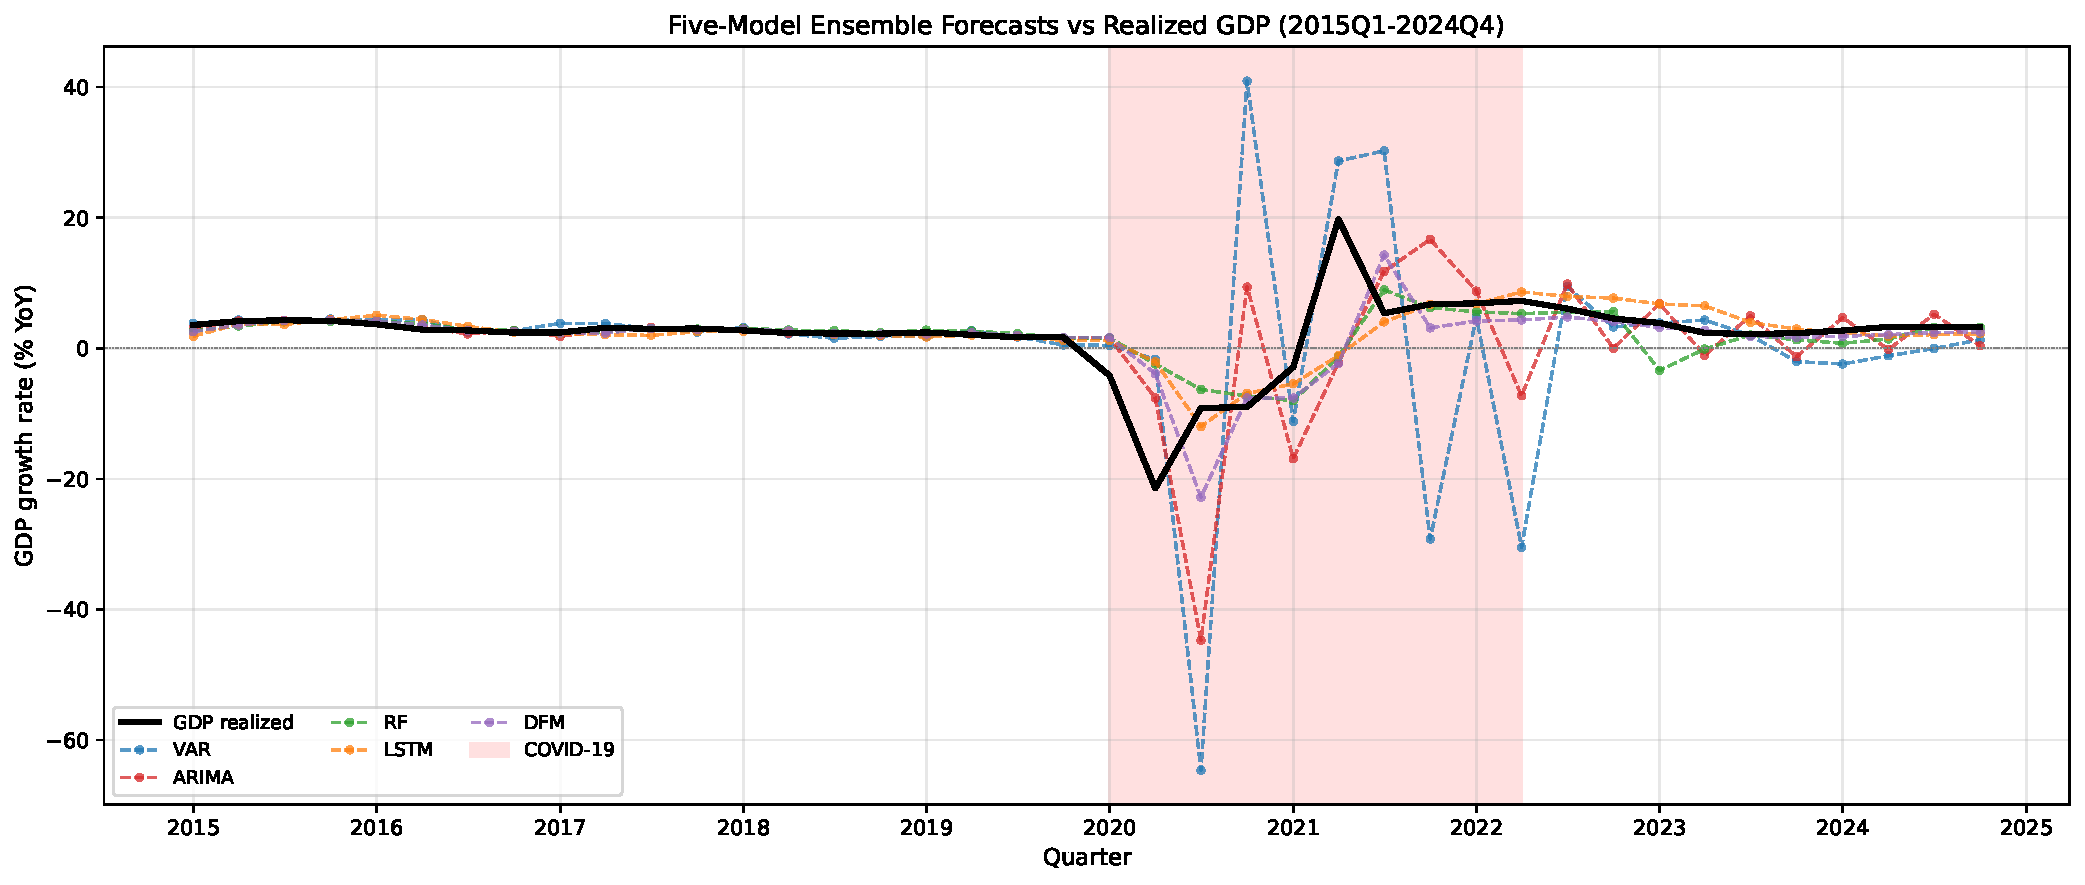
\includegraphics[width=0.85\textwidth]{figures/fig2_ensemble_forecasts.pdf}
    \caption{Five-Model Ensemble Forecasts vs. Realized GDP growth (2015Q1--2024Q4). The red shaded region indicates the COVID-19 crisis period (2020Q1--2022Q2).}
    \label{fig:ensemble_forecasts}
\end{figure}

\section{The Real-Time Uncertainty Index}
\label{sec:ceui_index}

We interpret the forecasting ensemble as an information-processing system. When the economic environment is stable, models converge and errors remain bounded; when a structural shock occurs, the system's internal disorder increases. The information-theoretic motivation is given in Appendix~A; here we describe the three observable, real-time measures that the framework maps onto. At each quarter $t$ we compute:

\begin{enumerate}
    \item \textbf{Within-model variability} ($\mathcal{U}^{\text{within}}_t$): the average, across models, of the trailing 4-quarter standard deviation of each model's recent forecast errors. It proxies how noisy each model has been about its own predictions. (As discussed in Appendix A, under a Gaussian approximation this dispersion is monotonically related to the average predictive entropy of the ensemble; the operational measure is the error-based standard deviation, not the theoretical quantity.)
    \item \textbf{Between-model dispersion} ($\mathcal{U}^{\text{between}}_t$): measures the disagreement among competing modeling paradigms. It is proportional to the empirical standard deviation of the point forecasts across the five models.
    \item \textbf{Temporal instability} ($\mathcal{U}^{\text{temporal}}_t$): captures the rate at which beliefs are updated between consecutive periods. It is computed as the trailing volatility of the ensemble's forecast path.
\end{enumerate}

Each measure is backward-looking and computed under the expanding-window protocol described in Section 4. The between-model and temporal dimensions use only forecasts available at $t$; the within-model dimension is discussed in Appendix~\ref{sec:appendix_u_within}, where we also report a variant that avoids any use of the target's final realisation.

\subsection{The Composite Economic Uncertainty Index (CEUI)}
We construct the CEUI directly from the raw standard deviations of the three dimensions. At each quarter $t$, we observe $\mathcal{U}^{\text{within}}_t$, $\mathcal{U}^{\text{between}}_t$, and $\mathcal{U}^{\text{temporal}}_t$. Because we seek an index that avoids the look-ahead bias arising from full-sample normalisation, we define the baseline CEUI as the simple average of the raw dimensions:

\begin{equation}
\label{eq:ceui}
\text{CEUI}_t = \tfrac{1}{3}\, \mathcal{U}^{\text{within}}_t
              + \tfrac{1}{3}\, \mathcal{U}^{\text{between}}_t
              + \tfrac{1}{3}\, \mathcal{U}^{\text{temporal}}_t .
\end{equation}

By operating on the raw scale, the index reflects the absolute magnitude of percentage-point deviations in the forecast system, and---because every dimension is backward-looking---it is available in real time. This raw measure is used for all empirical evaluations. For illustration only, when graphing the historical evolution of the index we also report a normalised 0--100 version based on full-sample percentiles; this is strictly an ex-post descriptive transformation (see Appendix~B). Figure~\ref{fig:ceui_dimensions} displays the path of the three individual dimensions of uncertainty and the composite index over the sample period.

\begin{figure}[ht]
    \centering
    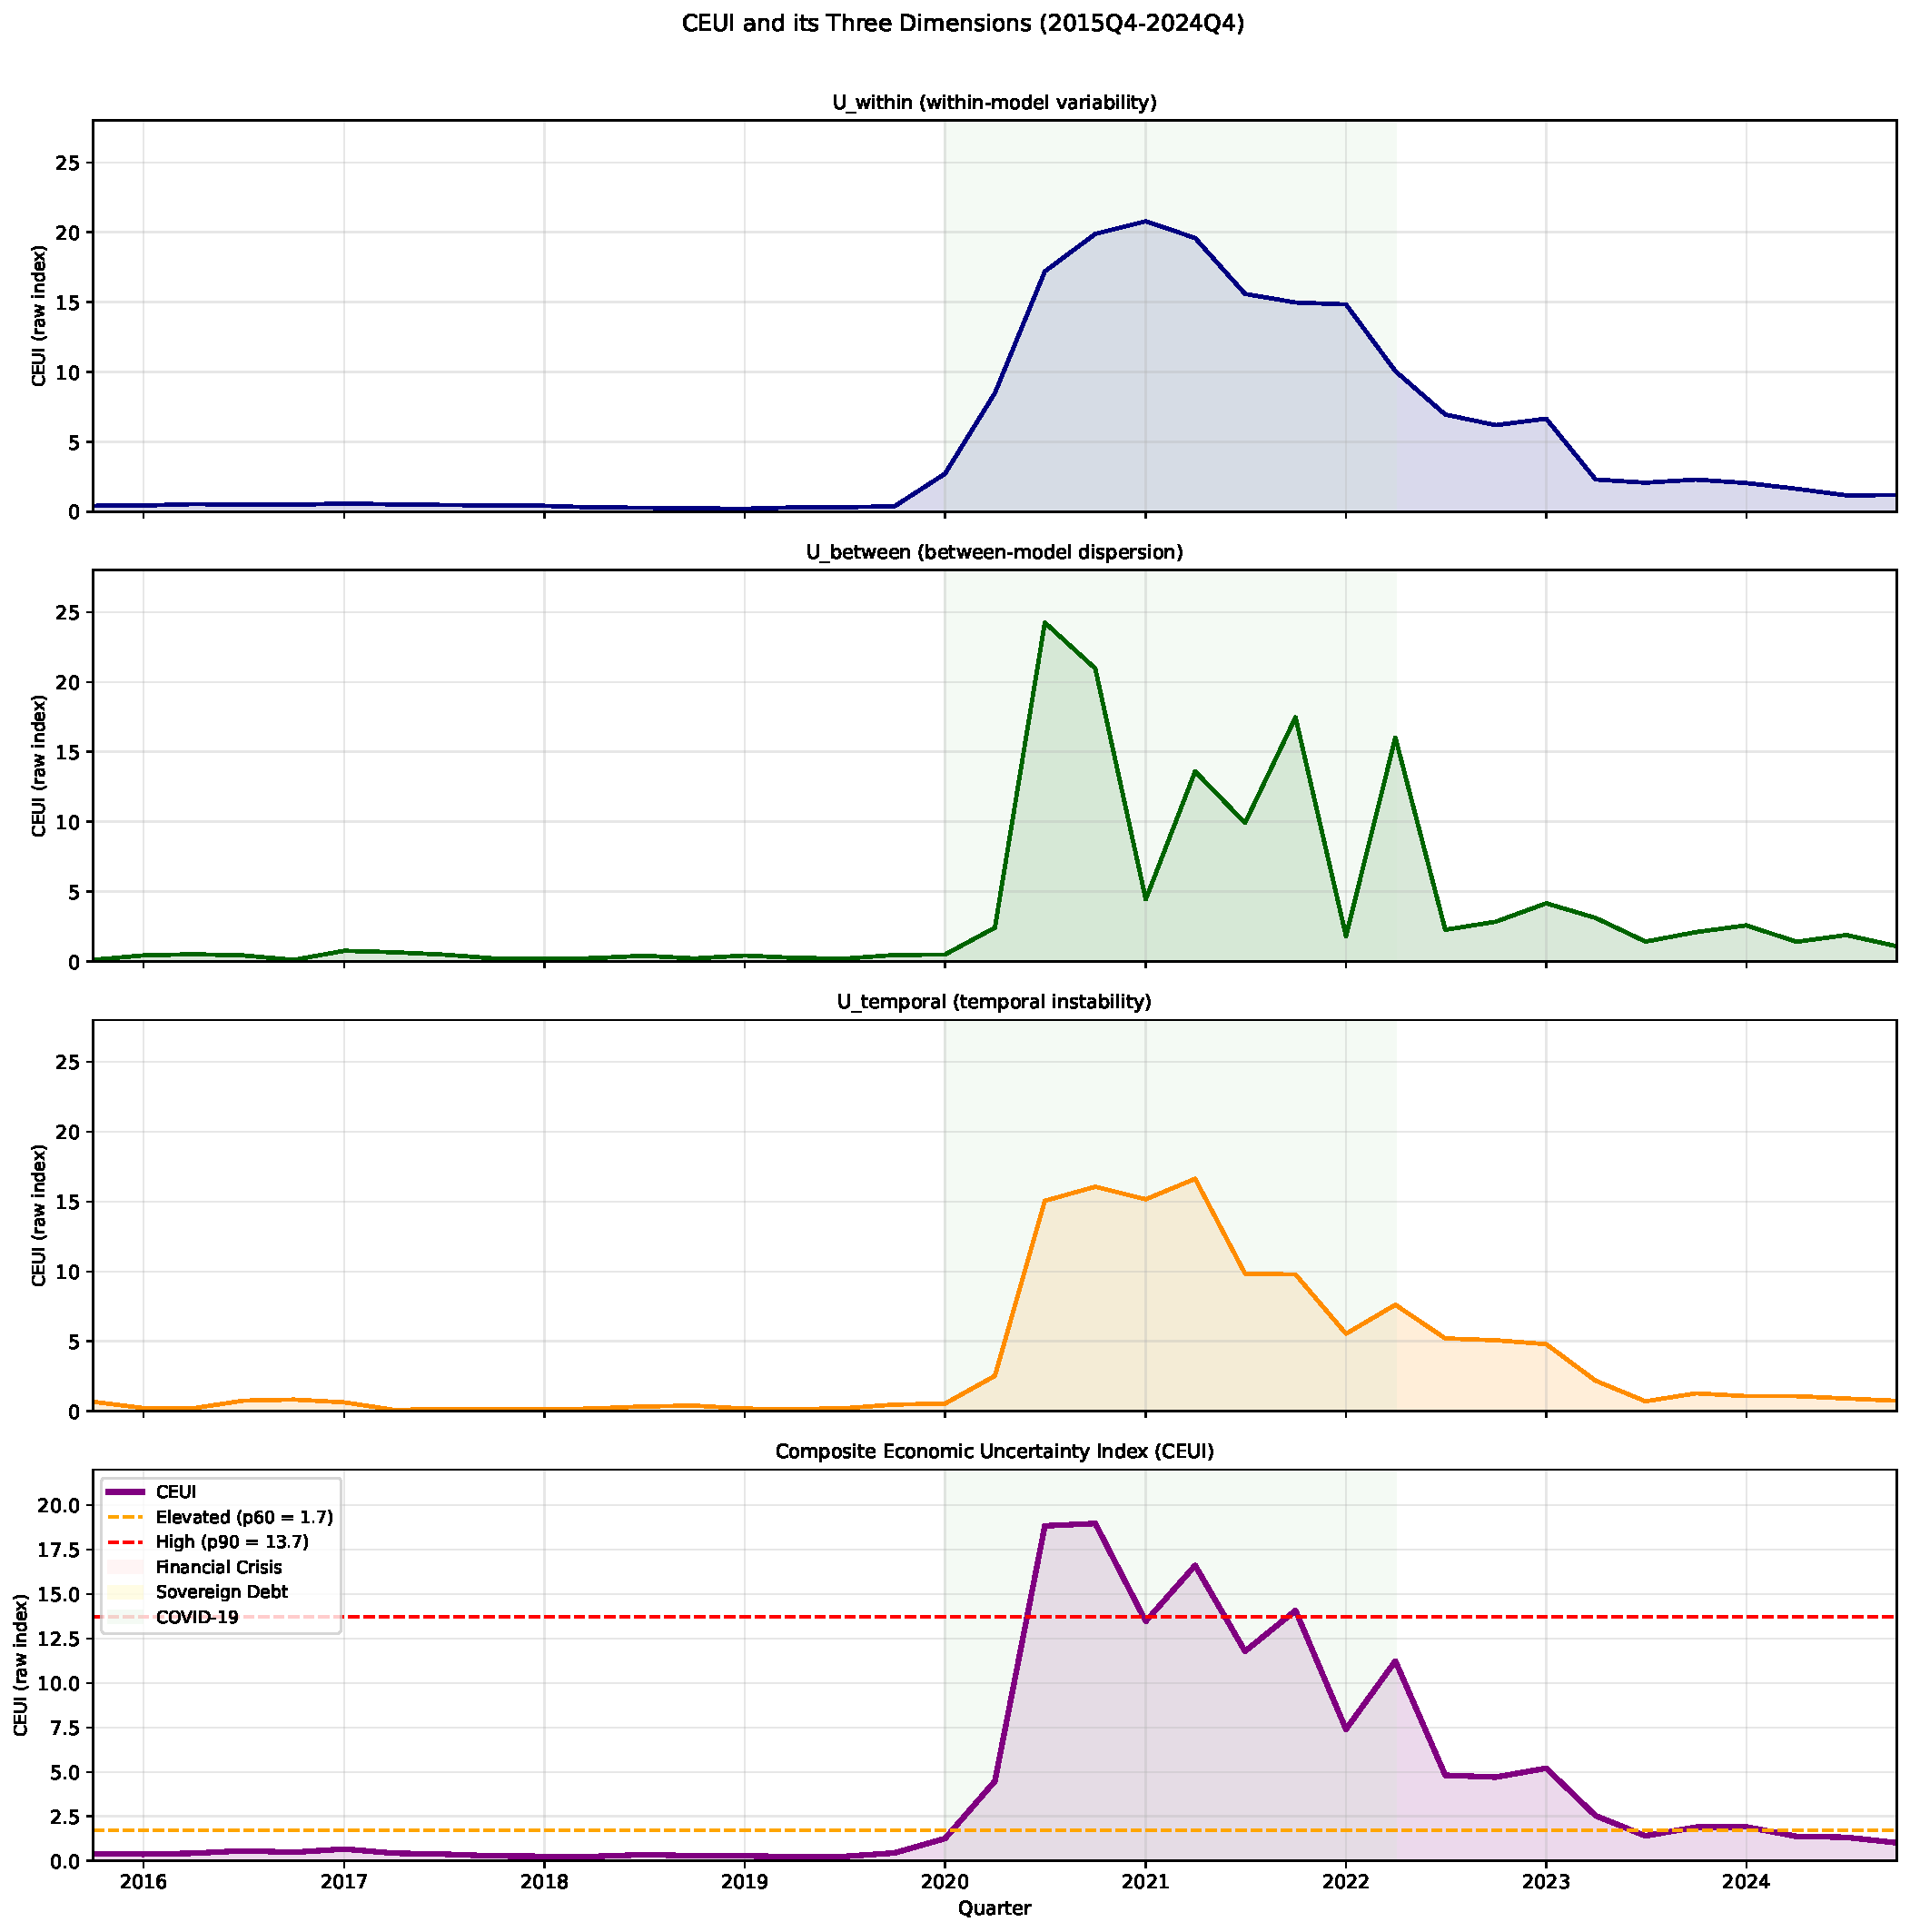
\includegraphics[width=0.85\textwidth]{figures/fig5_ceui_dimensions.pdf}
    \caption{Historical Path of the Three Uncertainty Dimensions and the Raw Composite Economic Uncertainty Index (CEUI) over 2015Q4--2024Q4.}
    \label{fig:ceui_dimensions}
\end{figure}

\section{Correlation of the CEUI with Revision Volatility}
\label{sec:correlation_volatility}

Our objective is to test whether the internal disorder of the forecasting ensemble ($\text{CEUI}_t$) is associated with the magnitude of the subsequent revision in the official GDP figure ($\sigma^{rev}_t$), which is the standard deviation of the revisions accruing to the quarter-$t$ estimate over the following two years. This two-year window is chosen to capture the bulk of the National Accounts regular revision cycle, which typically finalizes quarterly estimates after eight quarters. For the most recent quarters the two-year revision window is not yet complete; Appendix~\ref{sec:appendix_maturity} shows that controlling for vintage maturity leaves the association essentially unchanged ($\hat\beta = 0.0187$, $t = 2.89$).

We first estimate the baseline relationship between the CEUI and revision volatility by Ordinary Least Squares (OLS) with heteroscedasticity-robust (HC3) standard errors:
\begin{equation}
\label{eq:baseline}
\sigma^{rev}_t = \alpha + \beta \cdot \text{CEUI}_t + \varepsilon_t .
\end{equation}
Given our relatively small sample size ($N = 37$) and the presence of heavy-tailed observations during crisis periods, we rely on HC3 standard errors for inference in OLS, supplemented by the non-parametric Spearman rank correlation to ensure results are not driven solely by extreme outliers. Because the CEUI is calculated using data available strictly up to quarter $t$, it is a valid leading indicator for the revisions that unfold over the subsequent two years.

Empirically, we find a strong, positive association between the real-time CEUI and the magnitude of subsequent revisions. Over the 2015Q4--2024Q4 evaluation window ($N = 37$ quarters), the Spearman rank correlation between the index and revision volatility is $\rho = 0.727$ ($p < 0.001$). Estimating the baseline specification in Equation~\eqref{eq:baseline} yields a positive slope, $\hat{\beta} = 0.0198$ (SE $\approx 0.0064$), which is significant at the 1\% level under HC3-robust standard errors, explaining a substantial portion of the variance ($R^2 = 0.413$). 

To put the magnitude of this effect into context, consider the full observed range of the index, which spans from a minimum of approximately $0.25$ during calm periods to a peak of $18.88$ at the height of the COVID-19 pandemic. Over this range, the estimated slope implies a total shift of roughly $0.37$ percentage points ($\approx 0.0198 \times 18.63$) in revision volatility. This is an economically meaningful effect when compared to the baseline level of $\sigma^{rev}$ during quiet quarters (around $0.1$ pp) versus the highly turbulent COVID-19 quarters (around $0.6$ pp). 

Figure~\ref{fig:scatter} displays this relationship graphically. While the scatter plot shows a largely linear upward trend, one might be concerned that the result is entirely driven by the cluster of high-uncertainty observations during the pandemic. However, the sensitivity analysis reported in Table~\ref{tab:sensitivity} confirms that the positive slope is robust to sample selection. The association survives the complete exclusion of the core COVID-19 shock ($\hat{\beta} = 0.0297, p < 0.001$) and remains highly significant when omitting the single most influential observation, 2020Q3 ($\hat{\beta} = 0.0239, p < 0.01$). Thus, the informational entropy of the forecasting system provides a consistent signal of data unreliability across both normal and crisis periods.

\begin{figure}[ht]
\centering
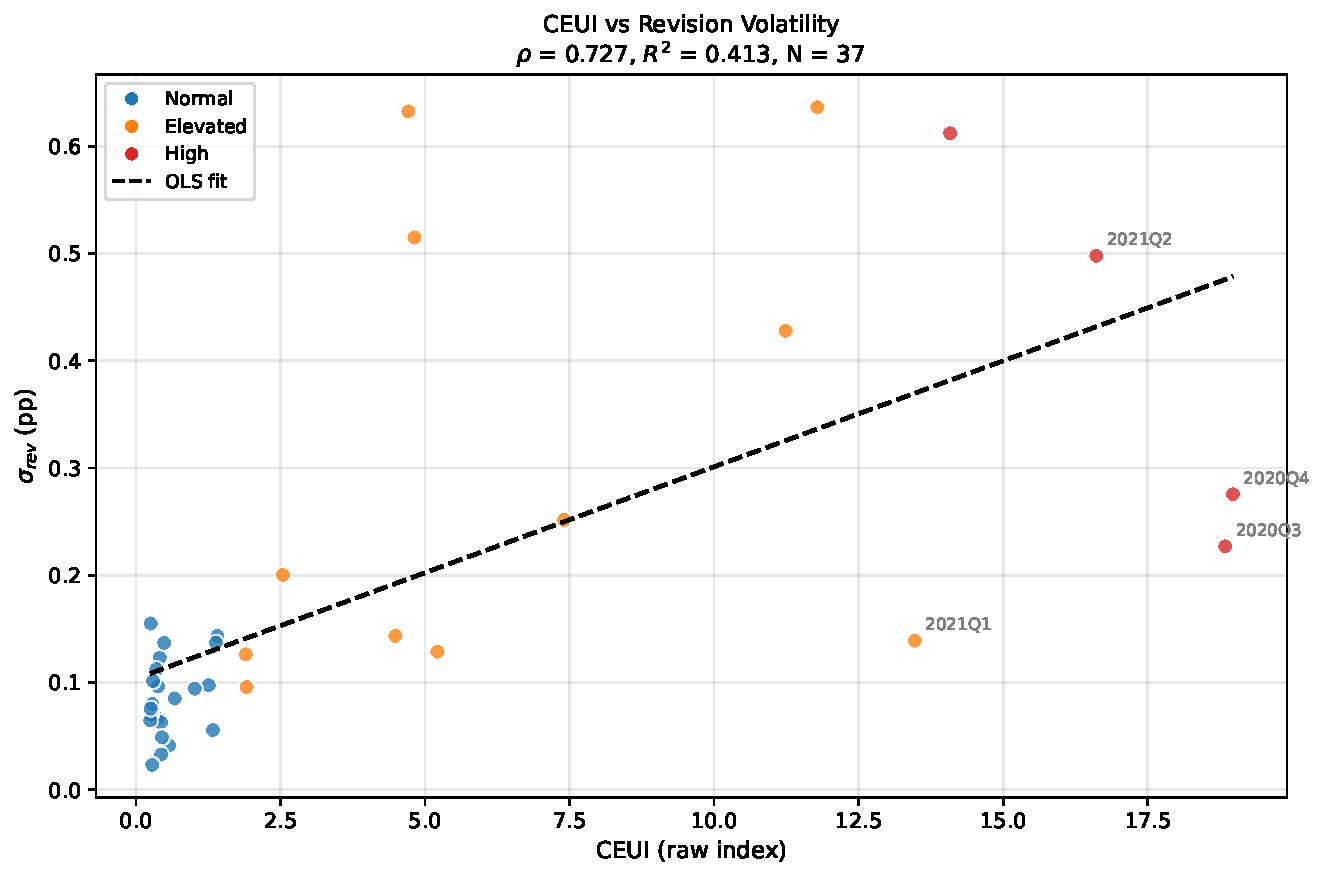
\includegraphics[width=0.72\textwidth]{figures/fig7_scatter_ceui_sigmarev.pdf}
\caption{Real-time CEUI versus the volatility of subsequent GDP revisions, 2015Q4--2024Q4 ($N = 37$). The fitted line corresponds to the baseline OLS specification in Equation~\eqref{eq:baseline}.}
\label{fig:scatter}
\end{figure}

\begin{table}[ht]
\centering
\begin{threeparttable}
\caption{Sensitivity of Baseline Regression across Subsamples}
\label{tab:sensitivity}
\begin{tabular}{lcccccc}
\toprule
Subsample & $\beta$ & $t$ & $p$ & $R^2$ & $\rho$ & $N$ \\
\midrule
Full sample & 0.0198 & 3.108*** & 0.0019 & 0.413 & 0.727 & 37 \\
Ex-COVID (2020Q2-Q4) & 0.0296 & 4.065*** & 0.0000 & 0.571 & 0.683 & 34 \\
Ex-crisis (2020Q1-2021Q1) & 0.0355 & 5.375*** & 0.0000 & 0.700 & 0.675 & 32 \\
Ex-most influential (2020Q3) & 0.0236 & 3.149*** & 0.0016 & 0.482 & 0.715 & 36 \\
\bottomrule
\end{tabular}

\begin{tablenotes}
  \small \item Note: HC3-robust standard errors. $^{***}p<0.01$, $^{**}p<0.05$, $^{*}p<0.10$.
\end{tablenotes}
\end{threeparttable}
\end{table}

To ensure that these results are not an artefact of the year-on-year (YoY) specification, we replicate this sensitivity analysis using quarter-on-quarter (QoQ) growth rates. Table~\ref{tab:sensitivity_qoq} reports these OLS regressions and Spearman correlations. The results are qualitatively identical to our baseline YoY findings. Over the full sample, the Spearman rank correlation between the CEUI and QoQ revision volatility is $\rho = 0.777$ ($p < 0.001$), which is slightly higher than the baseline YoY correlation ($\rho = 0.727$). The OLS coefficient on the CEUI is positive and statistically significant at the 5\% level ($\hat{\beta} = 0.0081, t = 2.062, p = 0.0392$), and excluding the full crisis window (2020Q1--2021Q1) yields a highly significant relationship outside the pandemic period ($R^2 = 0.473, t = 4.020, p < 0.001$). This confirms that the predictive link between our index and revision volatility is robust to the choice of the GDP growth specification. The corresponding QoQ ensemble forecasts and scatter plot are provided in Appendix~\ref{sec:appendix_qoq}.

\begin{table}[ht]
\centering
\begin{threeparttable}
\caption{Sensitivity of Baseline Regression under QoQ Growth Specification}
\label{tab:sensitivity_qoq}
\begin{tabular}{lcccccc}
\toprule
Subsample & $\beta$ & $t$ & $p$ & $R^2$ & $\rho$ & $N$ \\
\midrule
Full sample (QoQ) & 0.0081 & 2.062$^{**}$ & 0.0392 & 0.2226 & 0.777 & 37 \\
Ex-COVID (2020Q2--Q4) & 0.0114 & 0.899 & 0.3685 & 0.2677 & 0.738 & 34 \\
Ex-crisis (2020Q1--2021Q1) & 0.0237 & 4.020$^{***}$ & 0.0001 & 0.4727 & 0.698 & 32 \\
Ex-most influential & 0.0109 & 0.635 & 0.5255 & 0.2717 & 0.693 & 32 \\
\bottomrule
\end{tabular}

\begin{tablenotes}
  \small \item Note: HC3-robust standard errors. $^{***}p<0.01$, $^{**}p<0.05$.
\end{tablenotes}
\end{threeparttable}
\end{table}


To determine whether the CEUI captures information beyond standard uncertainty metrics, we also run a horse-race against the VIX (financial-market volatility) and the Economic Policy Uncertainty (EPU) index for Spain:
\begin{equation}
\label{eq:horserace}
\sigma^{rev}_t = \alpha + \beta_1 \text{CEUI}_t + \beta_2 \text{VIX}_t
               + \beta_3 \text{EPU}_t + \varepsilon_t .
\end{equation}
All predictors are standardised to mean zero and unit variance to allow direct comparison of the coefficients.

Table~\ref{tab:horserace} reports the horse-race regressions. We estimate Equation~\eqref{eq:horserace} over the sample for which the CEUI, the VIX, and the Spanish EPU series are jointly available ($N = 26$, 2015Q4--2022Q1), with the upper bound dictated by the EPU series available on policyuncertainty.com, standardising all predictors. Estimated individually, the CEUI is the strongest of the three predictors of revision volatility. While the VIX and EPU are powerful indicators of generalized risk (capturing market and political turbulence respectively), they often fail to predict revision volatility because they do not reflect the internal disorder of the statistical production system. In the individual models, the VIX and EPU explain only a small fraction of the variance in revision volatility ($R^2 = 0.057$ and $R^2 = 0.041$, respectively). By contrast, including the CEUI dramatically improves the model's explanatory power, driving the $R^2$ up to $0.565$ when all three are combined. In this joint specification, the CEUI remains highly significant, whereas the VIX and the EPU index become insignificant. The internal disorder of the forecasting ensemble therefore carries information about the reliability of official data that is not subsumed by market-based or news-based uncertainty measures---the paper's central empirical claim.

\begin{table}[ht]
\centering
\begin{threeparttable}
\caption{Horse-Race Regressions: CEUI vs VIX vs EPU as Predictors of Revision Volatility}
\label{tab:horserace}
\begin{tabular}{lcccccccc}
\toprule
 & \multicolumn{2}{c}{CEUI} & \multicolumn{2}{c}{VIX} & \multicolumn{2}{c}{EPU} & $R^2$ & $N$ \\
Specification & $\hat{\beta}$ & $t$ & $\hat{\beta}$ & $t$ & $\hat{\beta}$ & $t$ & & \\
\midrule
(1) CEUI only & 0.1206*** & 2.95 & -- & -- & -- & -- & 0.538 & 26 \\
(2) VIX only & -- & -- & 0.0392 & 1.49 & -- & -- & 0.057 & 26 \\
(3) EPU only & -- & -- & -- & -- & 0.0333 & 1.11 & 0.041 & 26 \\
(4) CEUI + VIX & 0.1307*** & 3.05 & -0.0217 & -1.17 & -- & -- & 0.552 & 26 \\
(5) CEUI + EPU & 0.1350*** & 3.16 & -- & -- & -0.0304 & -1.05 & 0.564 & 26 \\
(6) All three & 0.1346*** & 3.06 & 0.0030 & 0.12 & -0.0326 & -1.02 & 0.565 & 26 \\
\bottomrule
\end{tabular}

\begin{tablenotes}
  \small \item Note: Dependent variable $\sigma^{rev}_t$. All predictors standardised (zero mean, unit variance). HC3-robust $t$-statistics. $^{***}p<0.01$, $^{**}p<0.05$, $^{*}p<0.10$. Sample restricted to periods for which the CEUI, VIX, and Spanish EPU are jointly available ($N = 26$, 2015Q4--2022Q1), with the upper bound dictated by the available EPU series on policyuncertainty.com.
\end{tablenotes}
\end{threeparttable}
\end{table}

\section{Robustness Checks}
\label{sec:robustness}

To ensure the reliability of the baseline findings, we conduct several robustness checks focusing on real-time validity, alternative weighting schemes, model dependency, and normalization sensitivity.

First, we address the concern of look-ahead bias, a common critique of composite economic indices that utilize full-sample normalisation (whereby an index value at quarter $t$ depends on observations realised after $t$). Our baseline CEUI avoids this by construction: it is built from the raw, backward-looking dimensions, each of which uses only information available up to quarter $t$, requiring no full-sample rescaling. The headline association ($\rho = 0.727$) is therefore established under the quasi-real-time protocol, free of full-sample normalisation bias. The normalised 0--100 transformation used in the descriptive figures (Appendix~B) is an ex-post device that enters none of the estimates reported above; and because the central result is a rank correlation, it is invariant to any monotonic rescaling of the index. As a more demanding check, replacing the raw dimensions with their full-sample percentile-normalised counterparts---a transformation that does alter the composite's ranks---still yields $\rho = 0.727$, identical to the raw-index value and confirming that the central finding is not an artefact of the scaling choice.

Second, we verify that our results are not sensitive to the specific weights assigned to the three uncertainty dimensions. Table~\ref{tab:robustness_weights} presents CEUI variants constructed under four alternative weighting schemes. All alternative schemes achieve Pearson correlations above 0.997 with the equal-weight baseline and regime concordance above 97\%. These results confirm that the CEUI is virtually invariant to the choice of weights, primarily because the three dimensions share the dominant crisis signal. Equal weighting is retained as the baseline on grounds of parsimony and transparency.

\begin{table}[ht]
\centering
\begin{threeparttable}
\caption{Robustness to Alternative Weighting Schemes}
\label{tab:robustness_weights}
\begin{tabular}{lcccccc}
\toprule
Scheme & $w_{\text{within}}$ & $w_{\text{between}}$ & $w_{\text{temporal}}$ & Corr. baseline & Peak & Concordance \\
\midrule
Equal (Baseline) & 0.333 & 0.333 & 0.333 & 1.000 & 97.22 & 100.0\% \\
Dispersion-heavy & 0.200 & 0.500 & 0.300 & 0.997 & 97.22 & 97.3\% \\
Volatility-heavy & 0.500 & 0.300 & 0.200 & 0.997 & 97.22 & 100.0\% \\
Temporal-heavy & 0.200 & 0.300 & 0.500 & 0.997 & 97.22 & 100.0\% \\
\bottomrule
\end{tabular}

\begin{tablenotes}
  \small \item Note: Corr.\ baseline is the Pearson correlation with the equal-weight CEUI. Concordance is the percentage of periods where the regime classification (Normal, Elevated, High) matches the baseline. All correlations $> 0.99$.
\end{tablenotes}
\end{threeparttable}
\end{table}

Third, to ensure that the uncertainty signals are not driven by a single outlier model, we conduct a leave-one-model-out (LOO) analysis. By systematically excluding one model from the ensemble and recomputing the CEUI, we verify the stability of the aggregate index. As detailed in Table~\ref{tab:robustness_loo}, the LOO indices maintain very high correlations with the full ensemble, ranging from $0.818$ to $0.841$. Moreover, the predictive link with revision volatility is remarkably stable: the maximum change in the Spearman correlation ($\Delta\rho$) is merely $-0.029$ when the VAR model is excluded. This LOO analysis demonstrates that the structural features of the CEUI---particularly the crisis peaks and the correlation with official revisions---remain stable regardless of the specific composition of the model ensemble.

\begin{table}[ht]
\centering
\begin{threeparttable}
\caption{Leave-One-Model-Out (LOO) Ensemble Stability}
\label{tab:robustness_loo}
\begin{tabular}{lccc}
\toprule
Excluded model & Corr.\ with full ensemble & $\Delta$ Peak & $\Delta\rho_{\text{Spearman}}$ \\
\midrule
VAR & 0.824 & +78.250 & -0.039 \\
ARIMA & 0.840 & +77.324 & -0.012 \\
RF & 0.839 & +78.250 & -0.022 \\
LSTM & 0.841 & +78.250 & -0.018 \\
DFM & 0.838 & +77.324 & +0.002 \\
\bottomrule
\end{tabular}

\begin{tablenotes}
  \small \item Note: $\Delta\rho_{\text{Spearman}}$ measures the stability of the predictive link with revision volatility when one component is removed. The results confirm that no single model disproportionately drives the aggregate uncertainty signal.
\end{tablenotes}
\end{threeparttable}
\end{table}

Fourth, we check the sensitivity of our index to alternative scaling methods. Our baseline implementation uses raw dimensions for regression and percentile ranks to normalize the uncertainty components for graphical illustration. Table~\ref{tab:robustness_normalization} compares this approach with alternative scaling methods. Although the continuous correlations across normalisation methods are high ($0.891$ for percentile rank, $0.997$ for Z-score), the discrete regime classification is sensitive to the chosen scale (agreement ranges from $43.2\%$ to $59.5\%$ relative to the min-max baseline). This sensitivity reinforces our decision to rely on the continuous, unscaled index for all core regressions rather than on discrete regime thresholds.

\begin{table}[ht]
\centering
\begin{threeparttable}
\caption{Sensitivity to Normalization Methods}
\label{tab:robustness_normalization}
\begin{tabular}{lcc}
\toprule
Method & Corr.\ vs min-max & Regime agreement (\%) \\
\midrule
Percentile rank (baseline) & 0.891 & 43.2\% \\
Z-score & 0.997 & 59.5\% \\
Min-max [0,100] & 1.000 & 100.0\% \\
\bottomrule
\end{tabular}

\begin{tablenotes}
  \small \item Note: Regime Agreement measures the consistency of high-uncertainty flags across methods relative to the Min-Max baseline.
\end{tablenotes}
\end{threeparttable}
\end{table}

\section{Discussion}
\label{sec:discussion}

The empirical evidence supports a simple reading: when a panel of heterogeneous models disagrees and becomes unstable in real time, the official GDP figure released in that quarter is more likely to be substantially revised later. The mechanism driving this predictive power likely lies in a shared deterioration of the underlying informational environment. When primary, high-frequency data streams enter in a disorderly or conflicting manner, the forecasting models, which weigh inputs differently, naturally diverge. Simultaneously, the statistical agency's own triangulation of early data becomes inherently more fragile, leading to flash estimates that are prone to larger subsequent corrections once comprehensive survey data become available.

This finding bridges two distinct strands of literature. On one hand, \citet{aruoba2008} documents that GDP revisions are often heteroscedastic and not ``well-behaved,'' implying that data uncertainty varies over time. On the other hand, macroeconomic uncertainty measurement---exemplified by \citet{jurado2015} and \citet{baker2016measuring}---focuses on capturing periods when the economy becomes fundamentally harder to predict. The CEUI acts as a missing link between ex-ante forecasting uncertainty and ex-post statistical quality, showing that the internal entropy of the forecasting system provides a direct real-time proxy for the shifting variance of the data itself.

From a practical standpoint, the index offers a readily deployable tool for policymaking. Because the signal is available immediately and is built entirely from models an agency might already run internally, it does not depend on costly external financial data or complex text-mining algorithms. A statistical agency or government could use a high reading of the CEUI as an internal ``cautionary traffic light,'' signalling that the flash GDP estimate is unusually fragile. For governments making critical, often irreversible decisions—such as structural labor market reforms or aggressive fiscal consolidation plans—this index acts as a crucial real-time warning system. Proceeding with major policy shifts under the premise of high data uncertainty can lead to significant policy errors and welfare losses. Systematizing how policy should react to these warning signals represents a major area for quantitative analysis.

\paragraph{Model Resilience}
A secondary observation concerns model behaviour under extreme shocks. Linear models such as ARIMA, accurate in normal times, see their errors deteriorate sharply during crises, whereas the non-linear machine-learning components retain more adaptive capacity. This heterogeneity is what makes between-model dispersion informative; details are reported in Appendix~C.

\paragraph{Limitations}
Two qualifications shape the interpretation. First, the index predicts the \emph{volatility} of revisions, not their \emph{sign}: it flags fragile vintages, not the direction of the future correction. Furthermore, our evaluation window spans 2015Q4--2024Q4, yielding a small sample ($N = 37$). We mitigate this with heteroscedasticity-robust standard errors, but caution is warranted in extrapolation. The dominance of the COVID-19 pandemic in the sample means the index is heavily tested against one unprecedented shock. Additionally, the relationship could reflect a common confounding factor, where extreme macroeconomic volatility directly causes both forecast disagreement and measurement difficulties, rather than a direct causal chain. Finally, there is a recognized gap between theory and measurement: while information-theoretic entropy motivates the index conceptually, the operational measures are built from practical, backward-looking standard deviations.

\section{Conclusion}
\label{sec:conclusion}

We construct a Composite Economic Uncertainty Index (CEUI) from the internal statistics of a five-model forecasting ensemble for Spanish GDP, computed under a quasi-real-time, expanding-window protocol. The index is strongly associated with the subsequent volatility of official GDP revisions, and a horse-race shows that it carries predictive information beyond the VIX and the Spanish EPU index, both of which become insignificant once the CEUI is included. The measure offers statistical agencies, forecasters, and governments a transparent, real-time gauge of the reliability of early GDP estimates, built only from the internal properties of their own forecasting models. 

This index provides a practical foundation for policy analysis. Incorporating the CEUI into structural models stands as a natural and immediate direction for future research.

\section*{Declarations}

\subsection*{Funding}
The authors declare that no funding was received for this study.

\subsection*{Conflict of Interest}
The authors declare that they have no conflicts of interest.

\subsection*{Availability of Data and Materials}
The data supporting the findings of this study, including the CNTR real-time vintage database, are available in the public GitHub repository: \url{https://github.com/mhidper/entropia}.

\subsection*{Code Availability}
The replication code pipeline (Python) supporting this study is publicly available in the GitHub repository: \url{https://github.com/mhidper/entropia}.

\subsection*{Authors' Contributions}
Manuel Hidalgo-Pérez was the lead author and investigator. Leandro Navarro Pablo contributed to the empirical design and analysis. All authors read and approved the final manuscript.

\pagebreak
\section*{References} \label{sec:references}
\renewcommand{\bibsection}{}
\bibliographystyle{apalike}
\bibliography{bib}

\newpage
\appendix

\section{Information-Theoretic Foundations}
\label{sec:appendix_foundations}

This appendix gives the information-theoretic motivation for the three operational measures used in the body; the measures themselves are the backward-looking standard deviations defined in Section~3, and the development here is an approximation rather than an exact identity.

Treat the ensemble's quarter-$t$ forecast as a mixture of the five models' predictive densities, $p_t(y) = \tfrac{1}{M}\sum_{m=1}^{M} p_{m,t}(y)$ with $M = 5$. The Shannon entropy of this predictive distribution,
\begin{equation}
H(p_t) = -\int p_t(y)\log p_t(y)\,dy,
\end{equation}
is a natural scalar measure of the system's predictive disorder. A standard decomposition writes the entropy of the mixture as the average entropy of the components plus their Jensen--Shannon divergence \citep{haussler1997,heskes1998}:
\begin{equation}
H(p_t) \;=\; \underbrace{\tfrac{1}{M}\sum_{m} H(p_{m,t})}_{\mathcal{U}^{\text{within}}_t}
\;+\; \underbrace{\mathrm{JSD}\big(p_{1,t},\dots,p_{M,t}\big)}_{\mathcal{U}^{\text{between}}_t} .
\label{eq:decomposition_theory}
\end{equation}

The first term motivates the \emph{within-model} measure (how uncertain each model is about its own forecast) and the second the \emph{between-model} measure (how much the models disagree). To capture the dynamic dimension of uncertainty, we introduce a third component based on the informational distance between consecutive ensemble distributions: the Kullback--Leibler divergence of the current ensemble from the previous period's ensemble:
\begin{equation}
\mathcal{U}^{\text{temporal}}_t = D_{\text{KL}}(p_t \;\|\; p_{t-1}) = \int p_t(y) \log \frac{p_t(y)}{p_{t-1}(y)}\, dy .
\end{equation}

Under a Gaussian approximation, in which each model $m$ generates a predictive distribution $p_{m,t} = \mathcal{N}(\hat{y}_{m,t}, \sigma_{m,t}^2)$, these terms simplify as follows:

\begin{proposition}[Operational Equivalences under Gaussianity]
\label{prop:operational}
Under Assumption~G, the three components of predictive uncertainty satisfy:
\begin{enumerate}[label=(\roman*)]
    \item \textbf{Within-model uncertainty:}
    \begin{equation}
        \mathcal{U}^{\text{within}}_t = \frac{1}{M}\sum_{m=1}^{M} H(\mathcal{N}(\hat{y}_{m,t}, \sigma_{m,t}^2)) = \frac{1}{2}\ln(2\pi e) + \frac{1}{M}\sum_{m=1}^{M} \ln \sigma_{m,t}
    \end{equation}
    which is a monotone increasing function of the average log-predictive standard deviation.
    \item \textbf{Between-model dispersion:} Under homogeneous variance $\sigma_{m,t}^2 = \bar{\sigma}_t^2$ for all $m$, the Jensen--Shannon divergence satisfies:
    \begin{equation}
        \mathrm{JSD}\big(p_{1,t},\dots,p_{M,t}\big) \approx \frac{1}{2\bar{\sigma}_t^2} \cdot \frac{1}{M}\sum_{m=1}^{M}(\hat{y}_{m,t} - \bar{y}_t)^2
    \end{equation}
    where $\bar{y}_t$ is the cross-sectional mean of point forecasts. The JSD is thus proportional to the cross-sectional variance of point forecasts.
    \item \textbf{Temporal instability:} Considering consecutive Gaussian ensembles $p_t = \mathcal{N}(\bar{y}_t, \bar{\sigma}_t^2)$ and $p_{t-1} = \mathcal{N}(\bar{y}_{t-1}, \bar{\sigma}_{t-1}^2)$, the KL divergence takes the closed form:
    \begin{equation}
        \mathcal{U}^{\text{temporal}}_t = \frac{(\bar{y}_t - \bar{y}_{t-1})^2}{2\bar{\sigma}_{t-1}^2} + \frac{1}{2}\left(\frac{\bar{\sigma}_t^2}{\bar{\sigma}_{t-1}^2} - 1 - \ln\frac{\bar{\sigma}_t^2}{\bar{\sigma}_{t-1}^2}\right)
    \end{equation}
\end{enumerate}
\end{proposition}

This establishes that our operational measures (standard deviations and forecast differences) are direct proxies to theoretical entropy components.

\section{Uncertainty Regimes}
\label{sec:appendix_regimes}

While our main empirical results use the raw CEUI, classifying periods into discrete uncertainty regimes provides illustrative operational context. For this purpose we define the \textit{Normal} regime as CEUI $\leq$ p60, \textit{Elevated} as CEUI $\in$ (p60, p90], and \textit{High} as CEUI $>$ p90 based on the percentiles of the raw index (with full-sample values approximately p60 $\approx 1.69$ and p90 $\approx 13.62$). To preserve real-time validity, the percentiles are computed recursively using expanding windows. The 0--100 scale is used only for the illustrative figure, not for the tables. 

Table~\ref{tab:regime_table} shows the descriptive properties of the regimes, and Table~\ref{tab:threshold_stability} reports the stability of the thresholds under a bootstrap analysis. Figure~\ref{fig:regimes} shows the evolution of the CEUI and the uncertainty regimes.

\begin{table}[ht]
\centering
\begin{threeparttable}
\caption{Characteristics of Revisions by Uncertainty Regime}
\label{tab:regime_table}
\begin{tabular}{lcccccc}
\toprule
Regime & CEUI range & $N$ & $N_{rev}$ & MAE (pp) & vs Normal \\
\midrule
Normal & <= 1.7 & 22 & 22 & 0.087 & 1.0x \\
Elevated & 1.7-13.7 & 11 & 11 & 0.300 & 3.5x \\
High & > 13.7 & 4 & 4 & 0.403 & 4.7x \\
\bottomrule
\end{tabular}

\end{threeparttable}
\end{table}

\begin{table}[ht]
\centering
\begin{threeparttable}
\caption{Bootstrap Threshold Stability Analysis ($n = 1{,}000$)}
\label{tab:threshold_stability}
\begin{tabular}{lccccc}
\toprule
Threshold & Baseline & Boot mean & Boot std & \multicolumn{2}{c}{95\% CI} \\
 & & & & 2.5\% & 97.5\% \\
\midrule
Elevated (p60) & 1.70 & 2.12 & 1.21 & 0.63 & 4.78 \\
High (p90) & 13.72 & 13.32 & 3.13 & 5.21 & 18.84 \\
\bottomrule
\end{tabular}

\end{threeparttable}
\end{table}

\begin{figure}[ht]
\centering
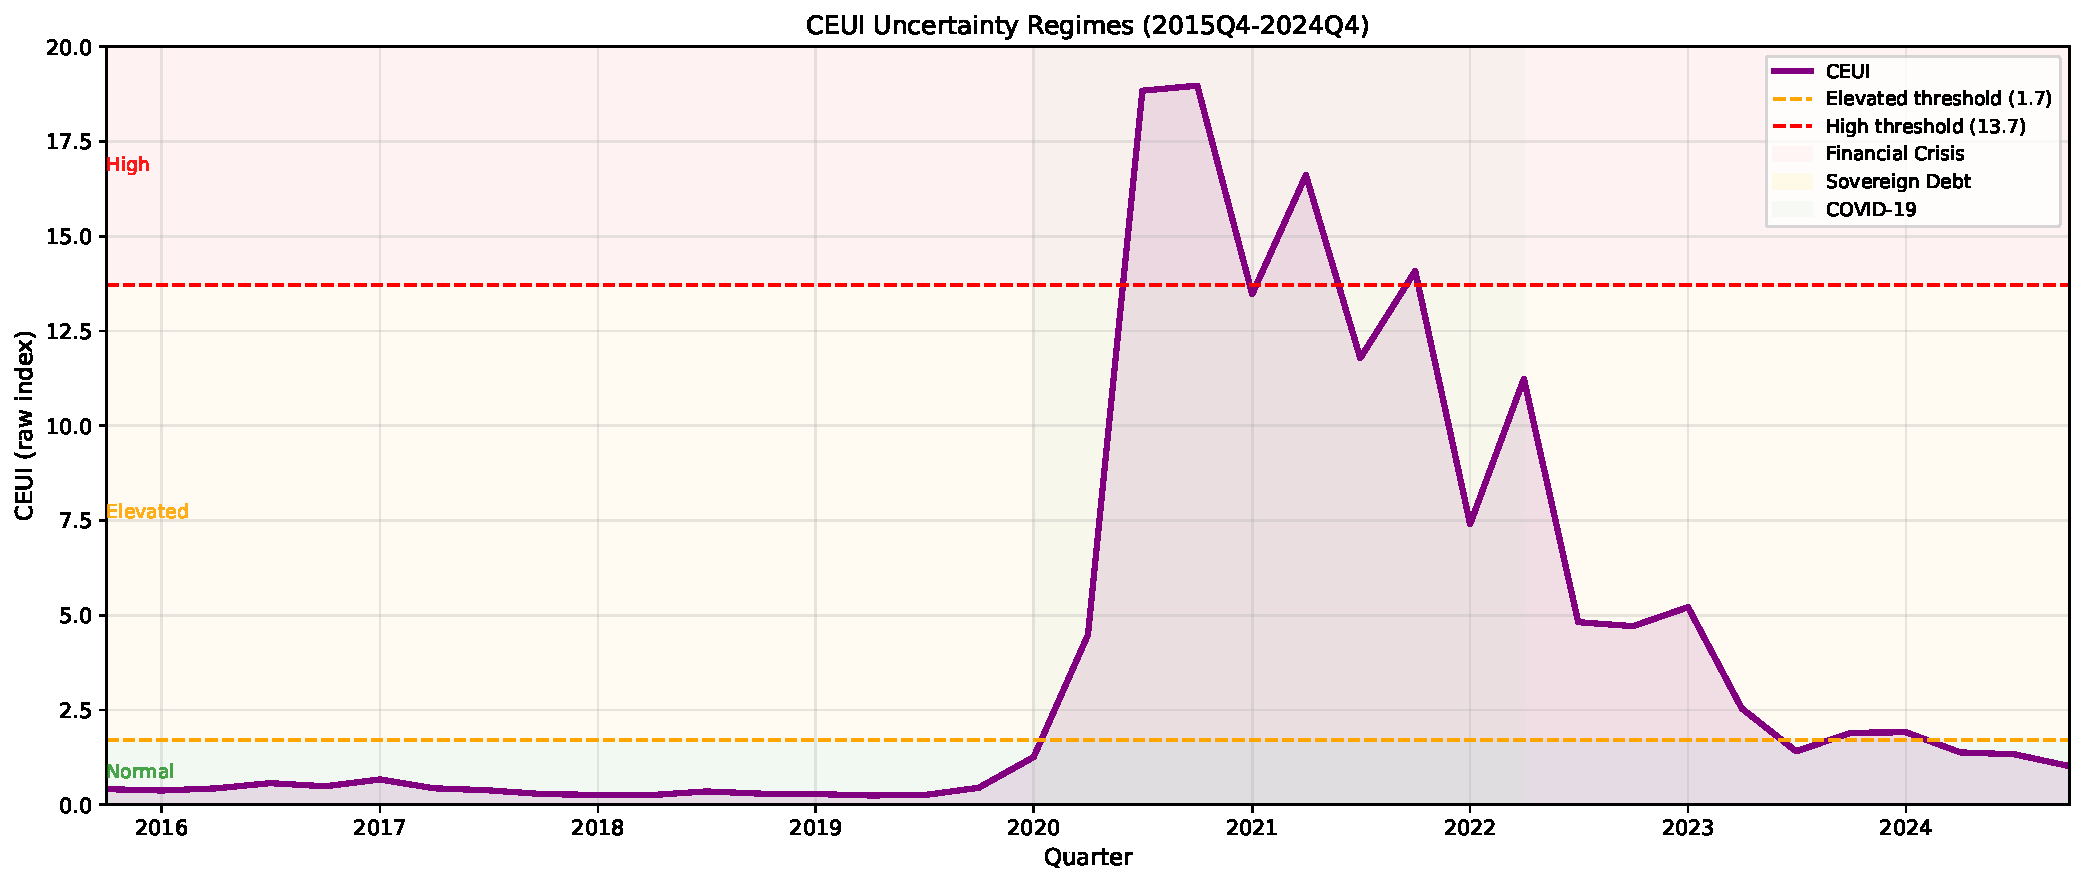
\includegraphics[width=0.8\textwidth]{figures/fig6_ceui_regimes.pdf}
\caption{CEUI evolution and recursive uncertainty-regime thresholds, 2015Q4--2024Q4.}
\label{fig:regimes}
\end{figure}

\section{Model Specifications and Resilience}
\label{sec:appendix_models}

The ensemble comprises five models estimated under an identical rolling protocol:
\begin{enumerate}
    \item \textbf{Vector Autoregression (VAR):} We implement a VAR system of 10 variables; the number of lags is selected recursively by AIC up to a maximum of 4.
    \item \textbf{Random Forest (RF):} The Random Forest implementation uses 100 trees with default depth, a fixed random seed (\texttt{random\_state=42}), and relies on 6 lags of GDP growth plus contemporaneous predictors.
    \item \textbf{ARIMA:} We employ a fixed ARIMA(4,0,1) specification on GDP growth.
    \item \textbf{Long Short-Term Memory (LSTM):} The LSTM architecture employs an 8-quarter input sequence, a single LSTM layer with 16 units, and is trained with early stopping (patience of 5 epochs).
    \item \textbf{Dynamic Factor Model (DFM):} We implement a DFM with a single common factor estimated using Kalman filtering and the EM algorithm.
\end{enumerate}

Table~\ref{tab:model_performance} compares the models' forecast accuracy in normal versus crisis periods, and Figure~\ref{fig:resilience} shows the ratio of crisis to normal-period forecast error.

\begin{table}[ht]
\centering
\begin{threeparttable}
\caption{Model Performance Summary (2019Q1--2024Q4)}
\label{tab:model_performance}
\begin{tabular}{lcccccc}
\toprule
Model & MAE & RMSE & MAE Normal & MAE Crisis & MAE ratio & Resilience \\
\midrule
VAR & 7.102 & 15.469 & 0.519 & 13.685 & 26.39x & 0.038 \\
ARIMA & 4.462 & 8.615 & 0.239 & 8.684 & 36.30x & 0.028 \\
RF & 2.176 & 4.920 & 0.384 & 3.968 & 10.33x & 0.097 \\
LSTM & 2.146 & 4.802 & 0.573 & 3.719 & 6.49x & 0.154 \\
DFM & 2.417 & 5.382 & 0.287 & 4.547 & 15.83x & 0.063 \\
\bottomrule
\end{tabular}

\end{threeparttable}
\end{table}

\begin{figure}[ht]
\centering
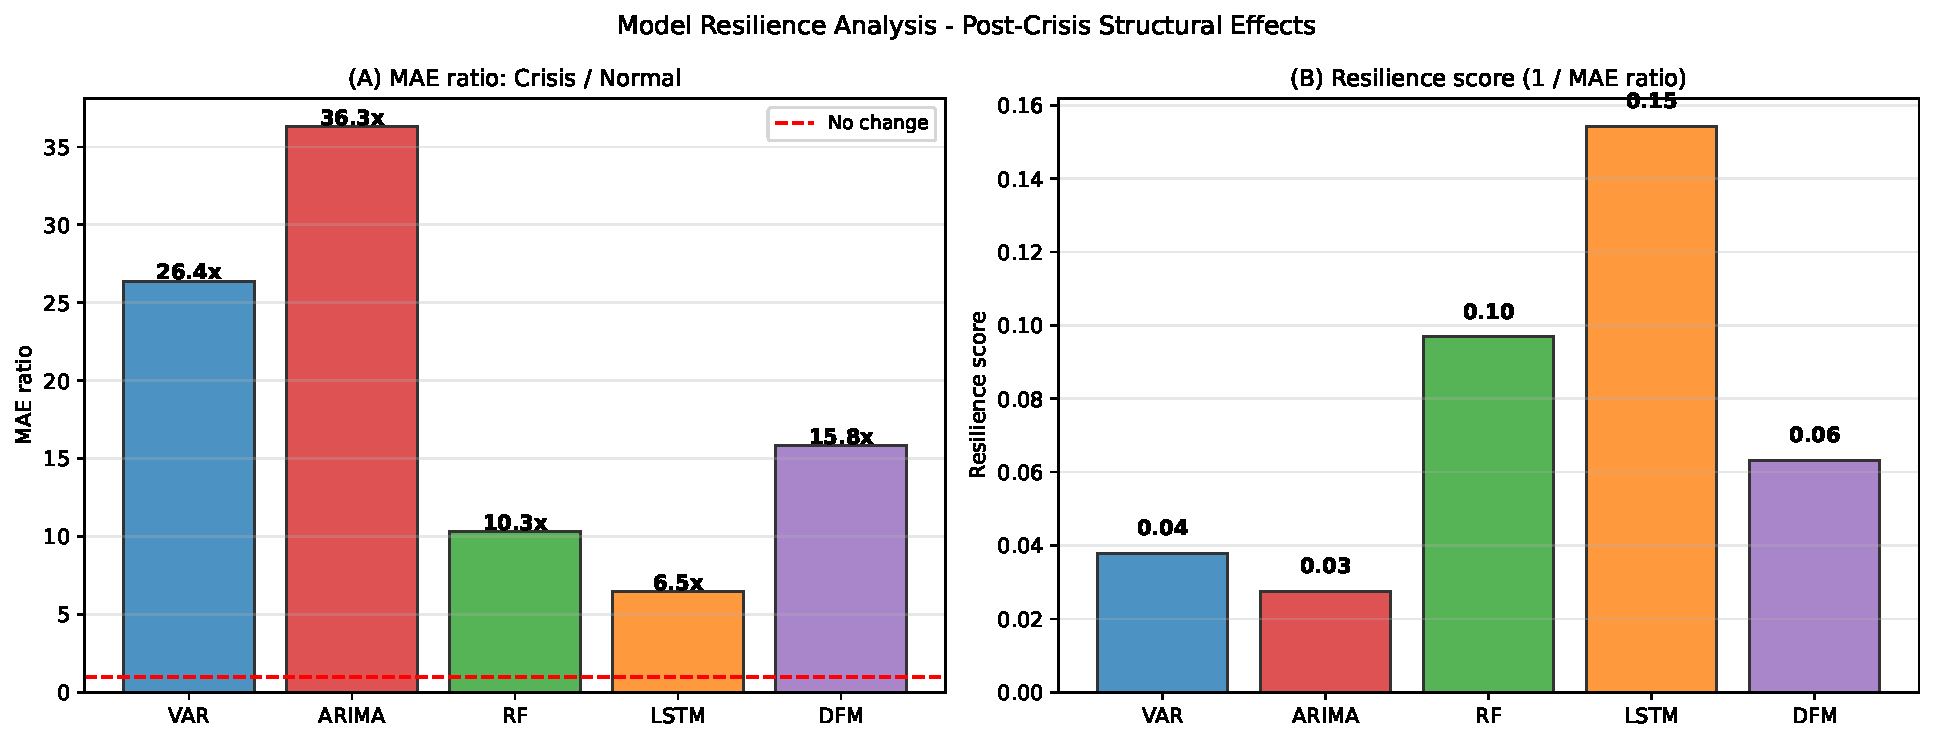
\includegraphics[width=0.8\textwidth]{figures/fig4_model_resilience.pdf}
\caption{Model resilience: ratio of crisis to normal-period forecast error by model.}
\label{fig:resilience}
\end{figure}

\section{Influence Diagnostics}
\label{sec:appendix_influence}

We report influence diagnostics for our baseline regression. Table~\ref{tab:influence_appendix} presents the diagnostic statistics, and Figure~\ref{fig:influence} displays the influence diagnostics. The results confirm that the positive association between the CEUI and revision volatility is not driven by any single observation: the maximum Cook's distance is $D = 0.556$ for 2020Q3.

\begin{table}[ht]
\centering
\begin{threeparttable}
\caption{Diagnostic Statistics for Influence Analysis}
\label{tab:influence_appendix}
\begin{tabular}{lcccccc}
\toprule
Quarter & CEUI & $\sigma_{rev}$ & Cook's $D$ & Leverage & Std.\ Resid. & Flagged \\
\midrule
2020Q3 & 18.84 & 0.2270 & 0.5494 & 0.2097 & -2.0352 & Yes \\
2020Q4 & 18.97 & 0.2756 & 0.3745 & 0.2130 & -1.6634 & Yes \\
2021Q3 & 11.79 & 0.6365 & 0.2147 & 0.0768 & 2.2715 & Yes \\
2021Q4 & 14.08 & 0.6120 & 0.1968 & 0.1109 & 1.7764 & Yes \\
2021Q1 & 13.47 & 0.1390 & 0.1761 & 0.1010 & -1.7704 & Yes \\
2022Q4 & 4.71 & 0.6325 & 0.1454 & 0.0274 & 3.2144 & Yes \\
2022Q3 & 4.82 & 0.5149 & 0.0768 & 0.0275 & 2.3315 & No \\
2021Q2 & 16.61 & 0.4978 & 0.0259 & 0.1587 & 0.5235 & No \\
2022Q2 & 11.24 & 0.4279 & 0.0224 & 0.0700 & 0.7714 & No \\
2017Q4 & 0.28 & 0.0233 & 0.0083 & 0.0391 & -0.6380 & No \\
\midrule
\multicolumn{7}{l}{Threshold: Cook's $D > 4/N = 0.1081$}\\
\bottomrule
\end{tabular}

\end{threeparttable}
\end{table}

\begin{figure}[ht]
\centering
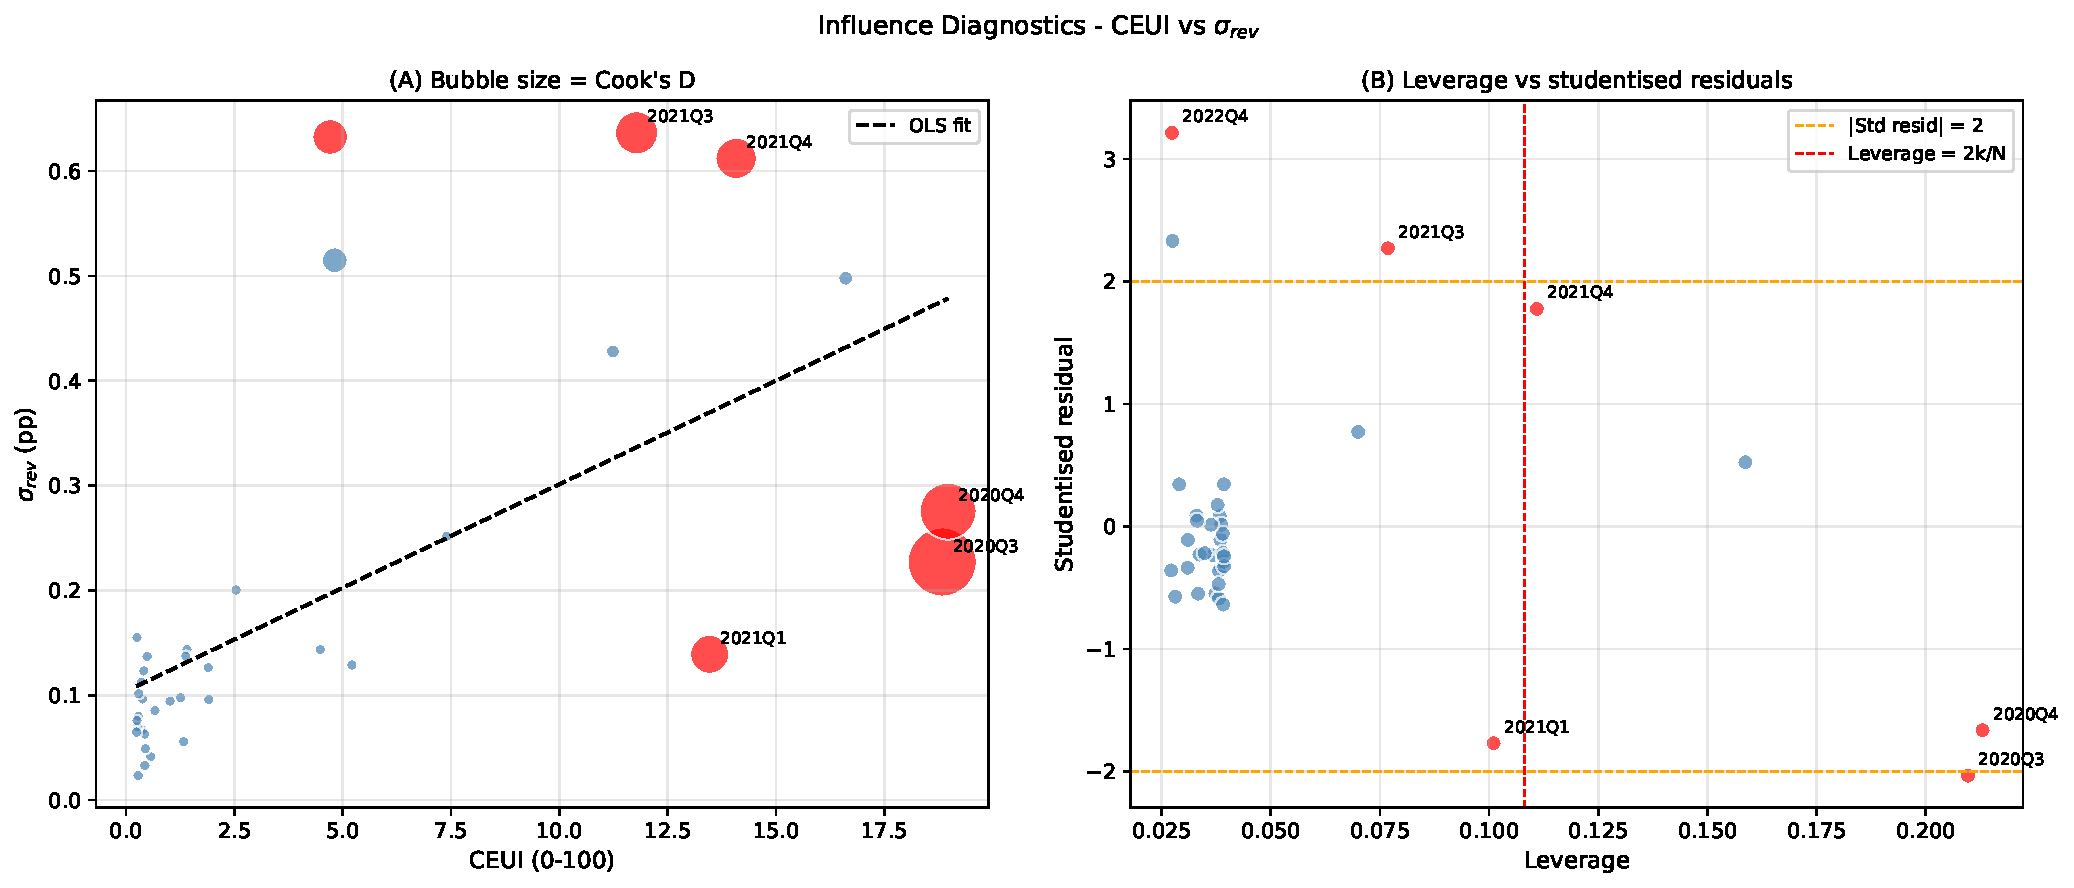
\includegraphics[width=0.8\textwidth]{figures/figA1_influence_diagnostics.pdf}
\caption{Influence diagnostics for the baseline regression (Equation~\eqref{eq:baseline}).}
\label{fig:influence}
\end{figure}

\section{VAR Specification Robustness}
\label{sec:appendix_var}

The main results are robust to the choice of VAR lag length and specification used in the ensemble. Table~\ref{tab:var_robustness} compares the baseline VAR(AIC selection, 10 variables) with a parsimonious VAR(2 lags, 4 core variables) model.

\begin{table}[ht]
\centering
\begin{threeparttable}
\caption{Robustness to Model Parsimony: Baseline vs Parsimonious VAR}
\label{tab:var_robustness}
\begin{tabular}{lccc}
\toprule
Specification & Avg.\ parameters & MAE (pp) & $\rho(\text{CEUI}, \sigma_{rev})$ \\
\midrule
VAR (AIC selection, 10 variables) & ~410 & 7.102 & 0.727 \\
VAR (2 lags, 4 core variables) & 36 & 4.322 & - \\
\bottomrule
\end{tabular}

\end{threeparttable}
\end{table}

\section{Vintage Maturity Control}
\label{sec:appendix_maturity}

The association survives controlling for the maturity of each vintage (the number of subsequent releases available), addressing the concern that more recent quarters mechanically display different revision behaviour. Table~\ref{tab:maturity_robustness} reports these regressions.

\begin{table}[ht]
\centering
\begin{threeparttable}
\caption{Robustness Check: Controlling for Vintage Maturity}
\label{tab:maturity_robustness}
\begin{tabular}{lccc}
\toprule
Variable & (1) Baseline & (2) Maturity control & (3) Excl.\ young ($vint < 8$) \\
\midrule
CEUI & 0.0198*** & 0.0185*** & 0.0195*** \\
 & (3.11) & (2.87) & (3.07) \\
$vint$ & -- & 0.0050 & -- \\
 & & (1.55) & \\
\midrule
$R^2$ & 0.413 & 0.423 & 0.405 \\
$N$ & 37 & 37 & 35 \\
\bottomrule
\end{tabular}

\end{threeparttable}
\end{table}

\section{Correlation Matrix}
\label{sec:appendix_correlation}

The three uncertainty dimensions are highly correlated with one another, which explains the near-invariance of the CEUI to alternative weighting schemes. Figure~\ref{fig:correlation_matrix} presents the pairwise Spearman correlations.

\begin{figure}[ht]
\centering
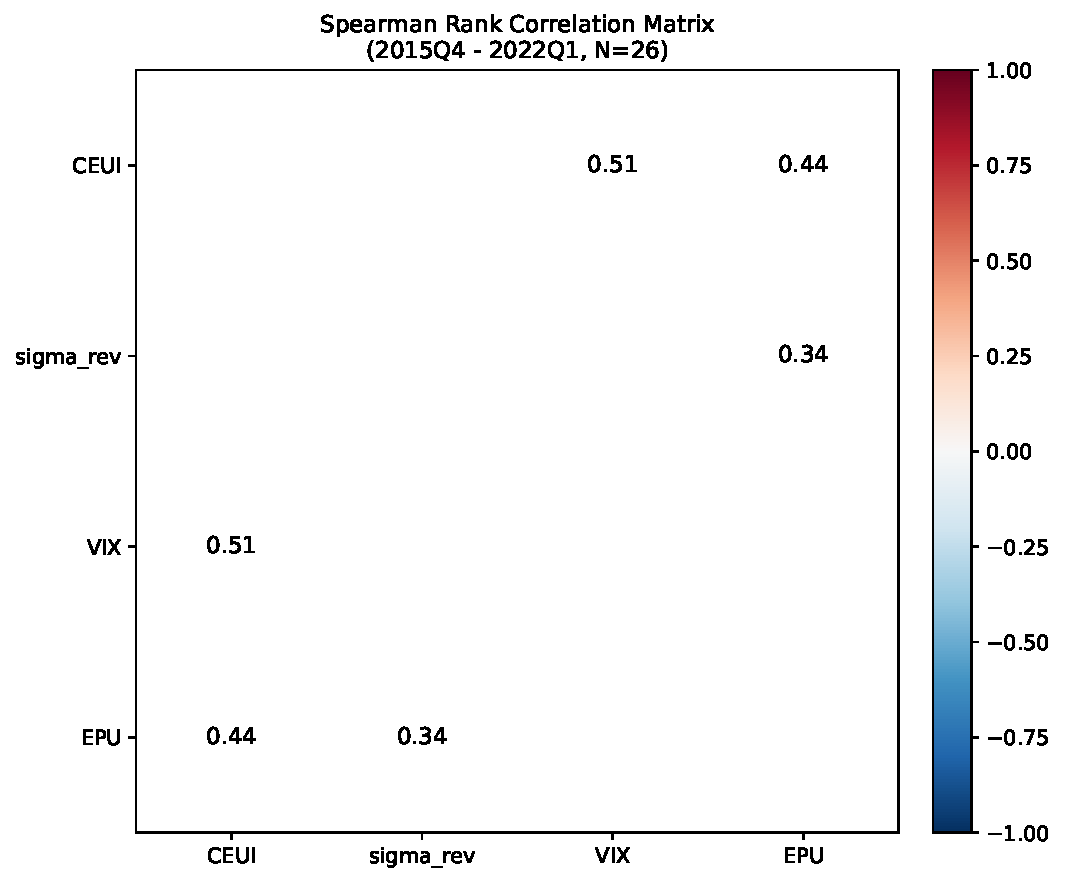
\includegraphics[width=0.8\textwidth]{figures/figD1_correlation_matrix.pdf}
\caption{Spearman rank correlations among the CEUI, revision volatility ($\sigma^{rev}$), and the external benchmarks (VIX and EPU), over the overlapping horse-race sample ($N = 26$, 2015Q4--2022Q1).}
\label{fig:correlation_matrix}
\end{figure}

\section{Robustness to Alternative GDP Growth Specifications (QoQ)}
\label{sec:appendix_qoq}

To ensure that our main empirical findings are not an artefact of the temporal smoothing or overlapping windows inherent in the year-on-year (YoY) specification, we replicate our entire analysis using quarter-on-quarter (QoQ) growth rates. Specifically, we redefine the target GDP growth rate as the percentage change relative to the preceding quarter ($t/t-1$). Correspondingly, the 7 non-stationary (I(1)) monthly indicators are also transformed into QoQ growth rates, while the stationary (I(0)) indicators (PMI and CLI) are kept in levels.

As detailed in Section~\ref{sec:correlation_volatility} (see Table~\ref{tab:sensitivity_qoq}), the OLS regressions and Spearman correlations under this QoQ specification yield results that are qualitatively identical to our baseline YoY findings. To supplement these results, Figure~\ref{fig:ensemble_forecasts_qoq} displays the out-of-sample forecasts of the ensemble against realized GDP growth in QoQ rates, showing that the models track the realized series in stable periods but diverge sharply during crises. Figure~\ref{fig:scatter_qoq} shows the scatter plot and fitted OLS regression line under the QoQ specification.

\begin{figure}[ht]
    \centering
    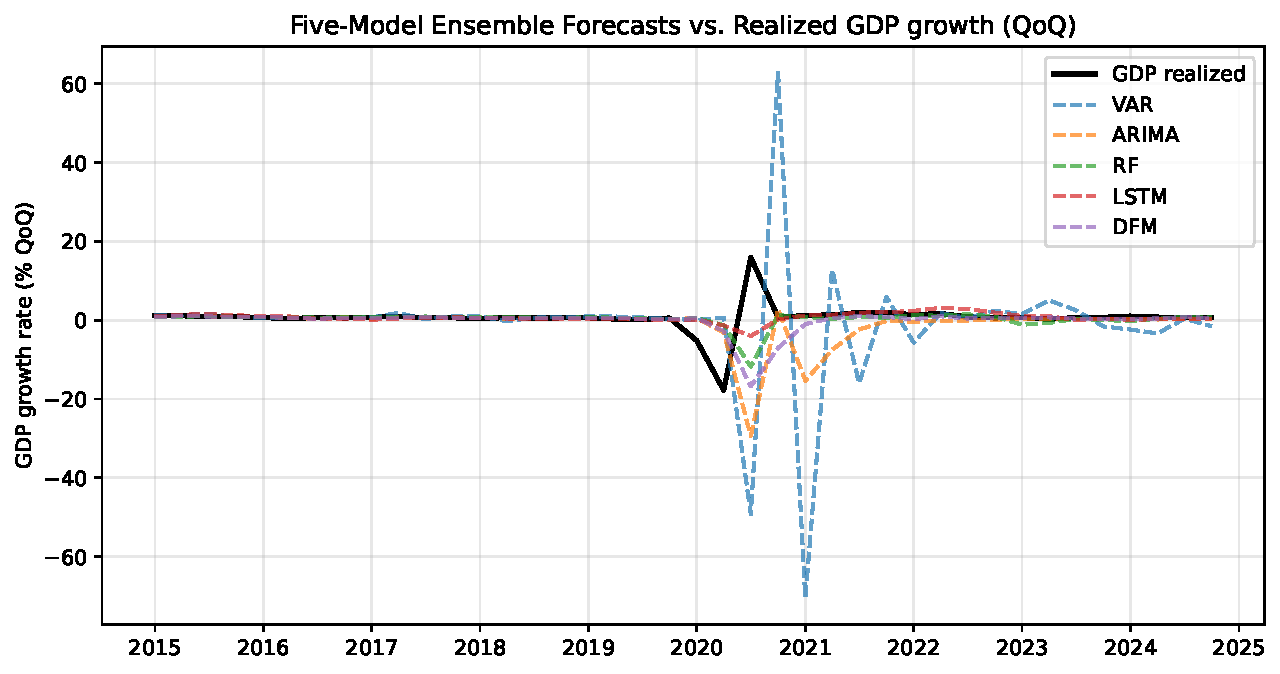
\includegraphics[width=0.85\textwidth]{figures/fig2_ensemble_forecasts_qoq.pdf}
    \caption{Five-Model Ensemble Forecasts vs. Realized GDP growth in QoQ rates (2015Q1--2024Q4).}
    \label{fig:ensemble_forecasts_qoq}
\end{figure}

\begin{figure}[ht]
    \centering
    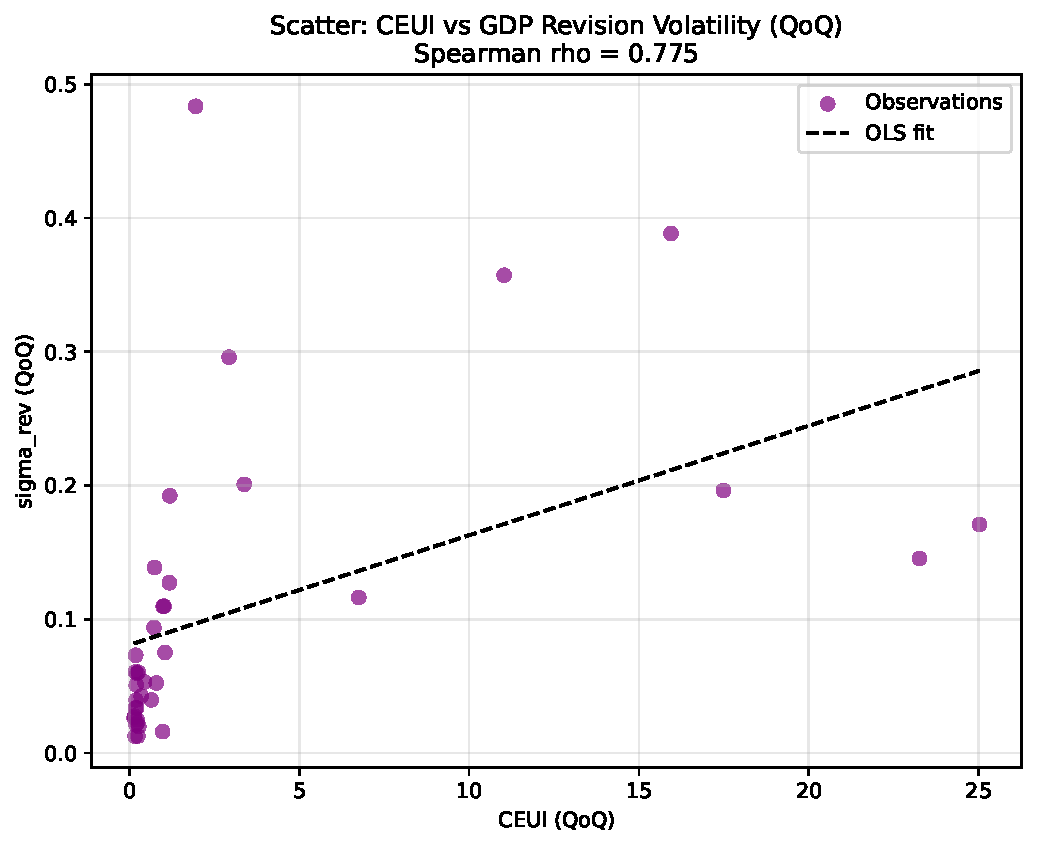
\includegraphics[width=0.72\textwidth]{figures/fig7_scatter_ceui_sigmarev_qoq.pdf}
    \caption{CEUI vs. GDP Revision Volatility under the QoQ specification.}
    \label{fig:scatter_qoq}
\end{figure}

\section{Robustness to In-Sample Within-Model Uncertainty}
\label{sec:appendix_u_within}

As a robustness check for the quasi-real-time implementation of the CEUI, we reconstruct the within-model dimension ($\mathcal{U}^{\text{within}}_t$) such that it avoids any use of the final realisation of the target quarter. In our baseline specification, the within-model standard deviation of forecast errors relies on comparing the out-of-sample prediction to the corresponding realisation. In this variant, we instead proxy the within-model uncertainty by calculating the standard deviation of each model's in-sample training residuals ($\mathcal{U}^{\text{within, train}}_t$). 

Substituting the baseline $\mathcal{U}^{\text{within}}_t$ with this in-sample variant yields a robust CEUI that does not depend on the availability of target realisations. The resulting index is virtually identical to the baseline, and its association with revision volatility remains equally strong: the Spearman rank correlation is $\rho = 0.734$ ($p < 0.001$), slightly higher than the baseline $\rho = 0.727$. This result is not driven by any single model: leave-one-model-out recomputations of the in-sample variant keep the Spearman correlation within [0.732, 0.739]. This confirms that our findings are not an artefact of the baseline index's partial reliance on contemporaneous error observations.

\end{document}
